%% LyX 2.3.5.2 created this file.  For more info, see http://www.lyx.org/.
%% Do not edit unless you really know what you are doing.
\documentclass[french]{article}
\usepackage[T1]{fontenc}
\usepackage[utf8]{inputenc}
\usepackage{geometry}
\geometry{verbose,tmargin=2cm,bmargin=2cm,lmargin=2.5cm,rmargin=2.5cm,headheight=1cm,headsep=1cm,footskip=1cm}
\setlength{\parskip}{\medskipamount}
\setlength{\parindent}{0pt}
\usepackage{float}
\usepackage{textcomp}
\usepackage{graphicx}

\makeatletter
%%%%%%%%%%%%%%%%%%%%%%%%%%%%%% User specified LaTeX commands.
\usepackage{listings}
\usepackage{xcolor}




\usepackage{babel}

\addto\extrasfrench{%
   \providecommand{\og}{\leavevmode\flqq~}%
   \providecommand{\fg}{\ifdim\lastskip>\z@\unskip\fi~\frqq}%
}




\makeatother

\usepackage{babel}
\makeatletter
\addto\extrasfrench{%
   \providecommand{\og}{\leavevmode\flqq~}%
   \providecommand{\fg}{\ifdim\lastskip>\z@\unskip\fi~\frqq}%
}

\makeatother
\begin{document}
\title{IFT 712 - Techniques d'apprentissage\\
 Projet de session}
\author{Étienne Ameye\\
 Yanni Mansour\\
 Djibril Sene}
\date{Lundi, 11 décembre 2023}

\maketitle
 

\pagebreak{}

\tableofcontents{}\pagebreak{}

\section{Méthodologie}

\subsection{Jeu de données}

Nous avons choisi le jeu de données de classification de feuilles
disponible sur Kaggle\footnote{https://www.kaggle.com/c/leaf-classification}.
Ce jeu de données contient 990 images de feuilles de 99 espèces différentes.
De ces images ont été extraites 3 caractéristiques : la marge, la
forme et la texture. Chaque caractéristique est donnée comme un vecteur
de 64 dimensions, pour un total de 192 dimensions.

\subsection{Méthodes d'évaluation}

Nous avons choisi de tester les classifieurs suivants : 
\begin{itemize}
\item Un classifieur KNN 
\item Un classifieur logistique 
\item Une machine à vecteur de support 
\item Un classifieur AdaBoost 
\item Un arbre de décision 
\item Une forêt aléatoire 
\end{itemize}
Afin de bien évaluer les performances de chaque classifieur, nous
avons séparé notre jeu de données en un ensemble d'entrainement et
un ensemble de test. Puisque notre jeu de données contient très peu
de données par classe, nous avons fait une séparation stratifiée.
De cette façon, on est garanti d'avoir autant de données dans chaque
classe. La figure \ref{fig:Distribution-des-classes} montre la différence
entre une séparation non stratifiée et une séparation stratifiée.
Cette différence dans la distribution des classes pourrait mener à
des biais lors de l'entrainement ou de l'évaluation.
\begin{center}
\begin{figure}[h]
\begin{centering}
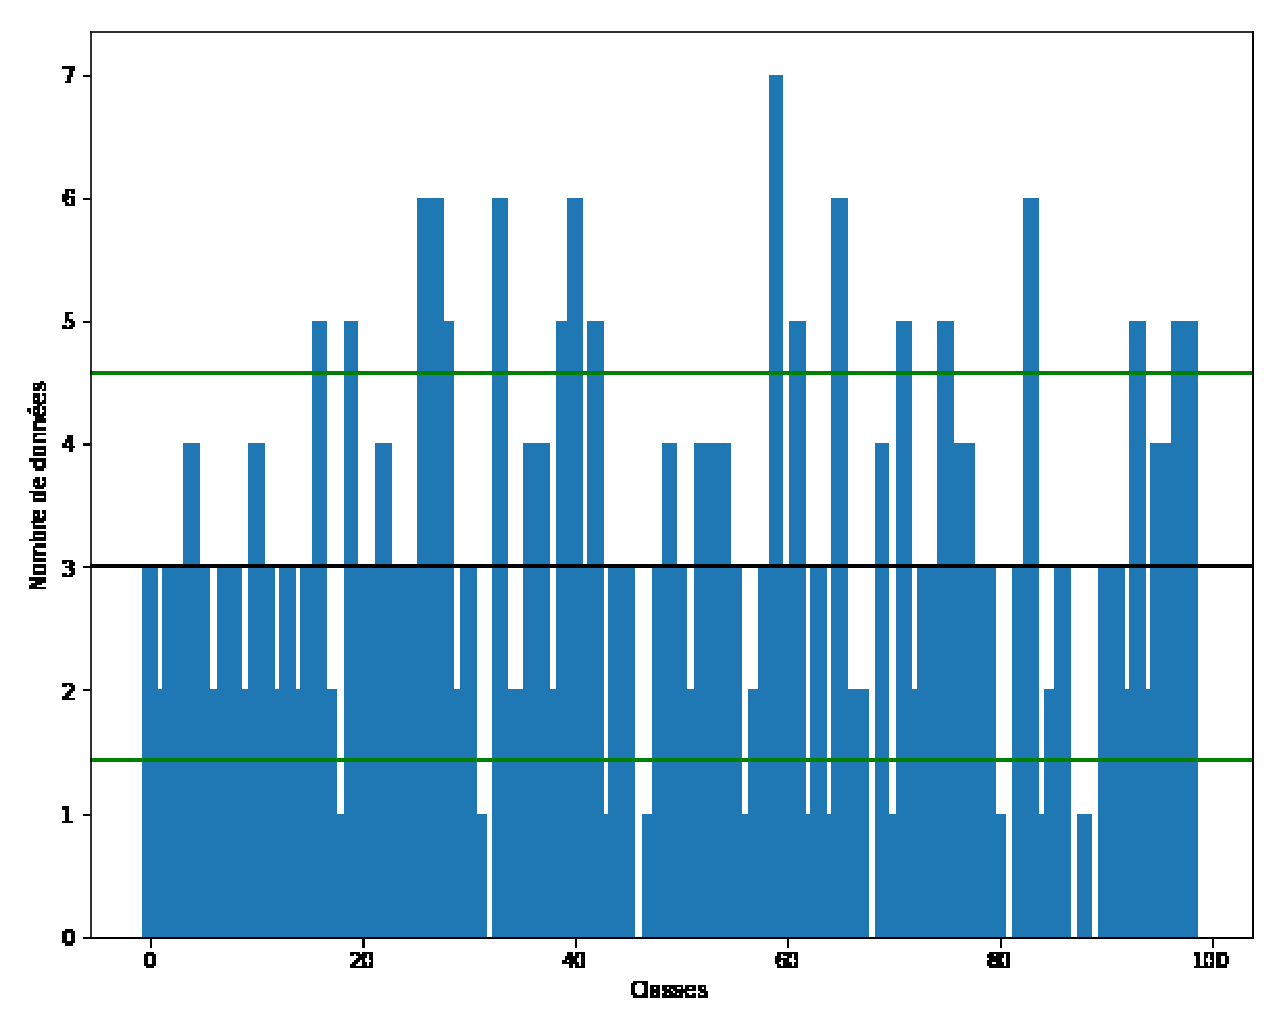
\includegraphics[scale=0.3]{images/class_distribution_unstratified}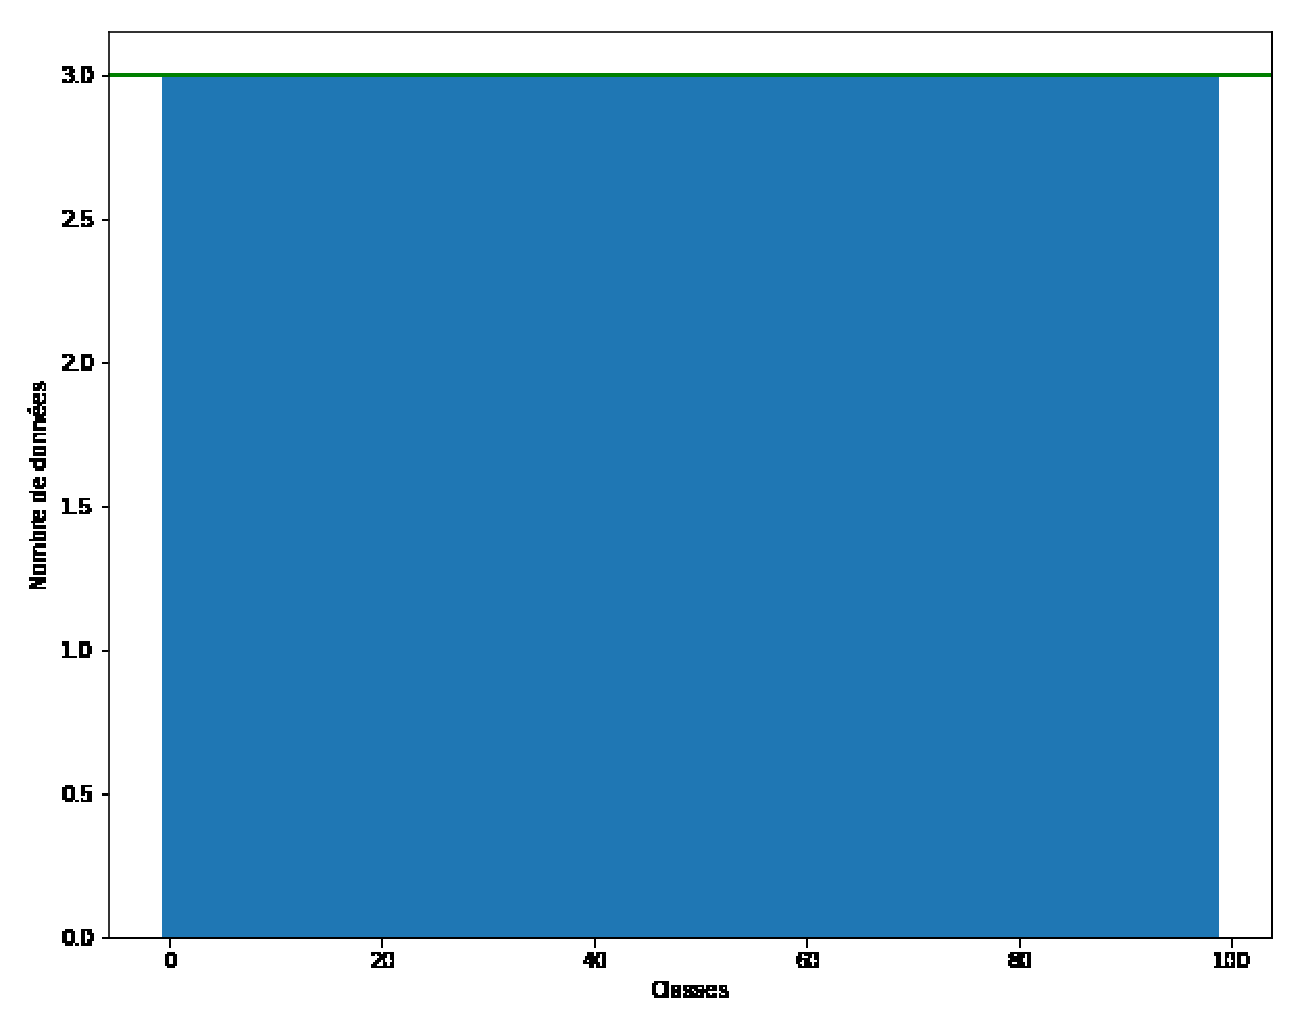
\includegraphics[scale=0.3]{images/class_distribution_stratified} 
\par\end{centering}
\caption{\label{fig:Distribution-des-classes}Distribution des classes dans
l'ensemble de test avec une séparation non stratifiée (à gauche) et
stratifiée (à droite)}
\end{figure}
\par\end{center}

Tous les classifieurs ont été testés et entrainés sur les mêmes ensembles.
Afin d'être sur d'avoir les performances optimales pour chaque modèle,
nous avons fait une recherche d'hyperparamètres par validation croisée.
Pour s'assurer d'avoir au moins une donnée par classe dans chaque
pli, nous avons limité la validation croisée à seulement 5 plis.

Chaque classifieur a été entrainé avec les meilleurs hyperparamètres
trouvés puis testé sur notre ensemble de test. Nous évaluerons les
performances des modèles sur l'ensemble de test avec les 3 métriques
suivantes : 
\begin{itemize}
\item La précision : la proportion de données appartenant réellement à leur
classe prédite 
\item Le rappel : la proportion des données bien classées (la justesse des
prédictions pour une classe) 
\item Le f1-score : la moyenne harmonique de la précision et du rappel 
\end{itemize}
Comme nous sommes dans une situation de classification multi-classes,
on calcule ces métriques individuellement pour chaque classe. On peut
ensuite calculer la moyenne sur l'ensemble des classes ou regarder
la distribution des résultats pour chaque métrique. On devrait ainsi
avoir une bonne idée des performances de chaque classifieur.

\subsection{Structure du projet}

Le code relatif à chaque classifieur se trouve dans des \textit{notebooks}
différents. Nous avons regroupé les fonctions utilitaires communes
à chaque \textit{notebook} dans le fichier \textit{DataManagement.py}.
Ce fichier contient aussi la classe \texttt{Dataset} qui sert à la
lecture et à la gestion du jeu de données. Le jeu de données se trouve
dans le dossier \textit{data}, dans le fichier \textit{train.csv}.

\pagebreak

\section{Évaluation des résultats}

\subsection{Classifieur KNN}

Le premier classifieur que nous avons choisi de tester est le KNN.
Il s'agit d'un classifieur qui prédit la classe d'une donnée selon
les classes des données qui se trouve autour (qu'on appelle les voisins).
L'avantage de ce classifieur est qu'il est simple et qu'il possède
peu d'hyperparamètres. Il est donc assez facile à optimiser. Par contre,
il peut avoir tendance à sur-apprendre les données d'entrainement.
On s'attend à un bon résultat avec ce classifieur parce qu'on suppose
que les feuilles doivent être significativement différentes d'une
espèce à l'autre.

Les hyperparamètres du KNN sont les suivants : 
\begin{itemize}
\item Le nombre de voisins 
\item La pondération associée à chaque voisin : uniforme (sans pondération)
ou selon la distance 
\item La métrique de distance : euclidienne, manhattan ou cosinus 
\end{itemize}
L'hyperparamètre le plus important est évidemment le nombre de voisin;
c'est lui qui détermine vraiment la capacité du modèle.

Les meilleurs hyperparamètres pour notre ensemble d'entrainement sont
: 
\begin{itemize}
\item Nombre de voisins : 4 
\item Pondération : selon la distance 
\item Métrique de distance : manhattan 
\end{itemize}
La figure \ref{fig:Score-du-KNN} montre les résultats de l'entrainement
pour les différentes valeurs d'hyperparamètres. On remarque une différence
significative entre la distance de manhanttan et les deux autres,
ce qui est plutôt inattendu. On remarque aussi qu'une pondération
selon la distance est toujours meilleure qu'une pondération uniforme,
ce qui est logique si nos données sont assez bien séparées. 
\begin{center}
\begin{figure}[h]
\begin{centering}
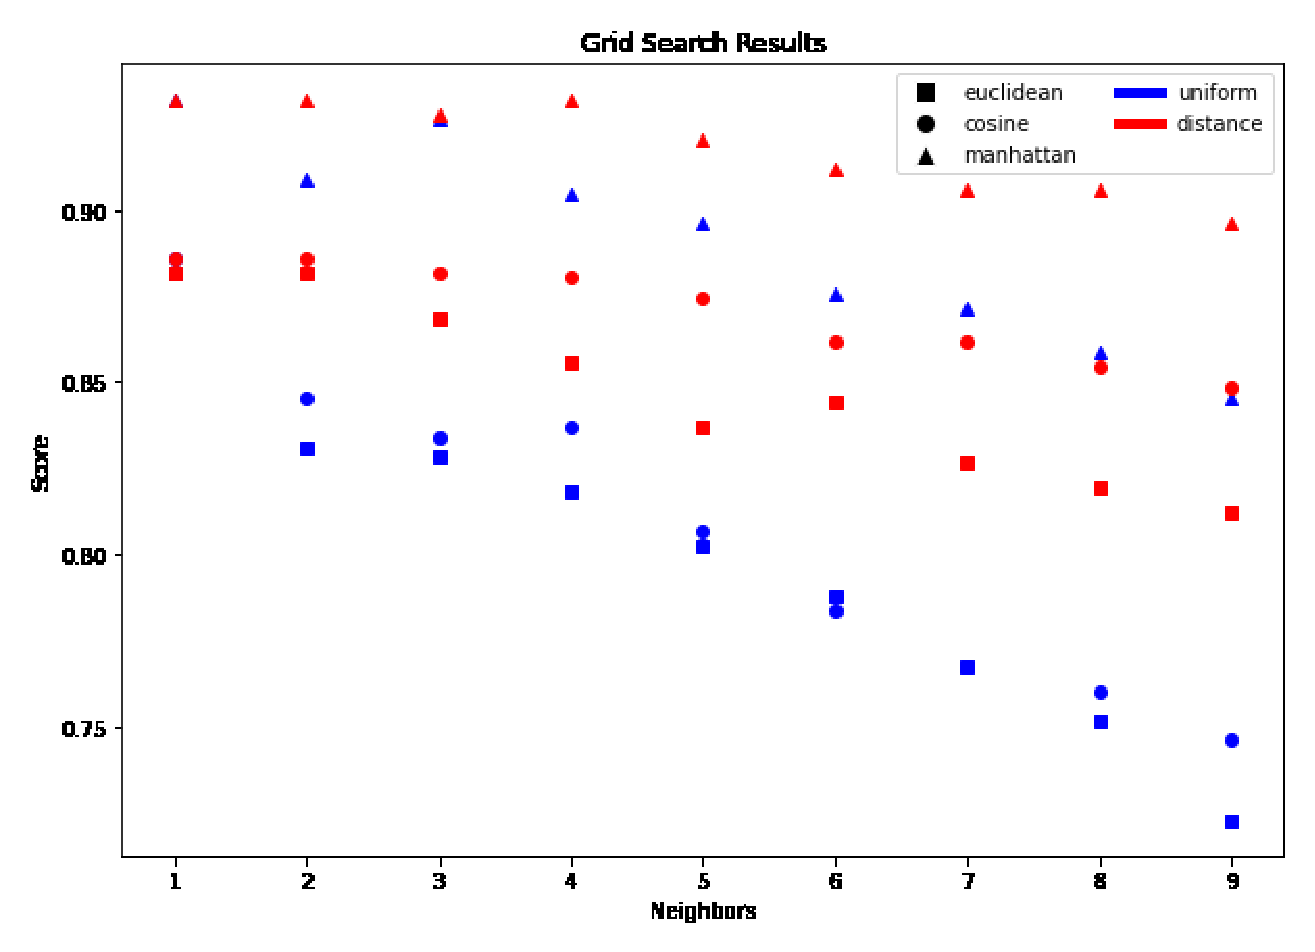
\includegraphics[scale=0.55]{images/knn_cross_validation} 
\par\end{centering}
\caption{\label{fig:Score-du-KNN}Score du KNN selon les différents hyperparamètres}
\end{figure}
\par\end{center}

On peut voir sur le graphique que le score est décroissant lorsqu'on
utilise plus que 4 voisins, et ce peu importe la distance ou la pondération.
Cette décroissance s'explique par le petit nombre de données dans
chaque classe dans l'ensemble d'entrainement. Plus on considère de
voisins, plus on considère de points qui n'appartiennent à la même
classe.\\
 Tout cela montre que nos données semblent assez bien séparées et
c'est pourquoi le classifieur KNN obtient un score aussi élevé.

Cependant, pour être sûr des performances du modèle, nous devons l'évaluer
sur l'ensemble de test. Pour chacune des métriques d'évaluation, voici
la moyenne calculée pour l'ensemble des classes sur les données de
test : 
\begin{itemize}
\item Précision : 96,397 \textpm{} 9,469 \% 
\item Rappel : 95,286 \textpm{} 13,477 \% 
\item F1-score : 95,005 \textpm{} 13,409 \% 
\end{itemize}
\begin{center}
\begin{figure}[h]
\begin{centering}
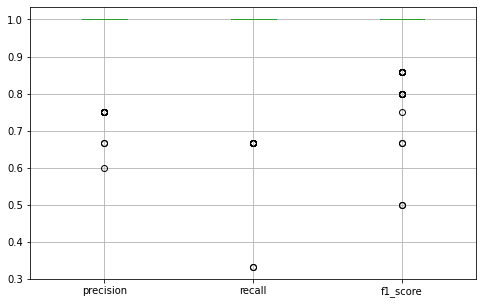
\includegraphics[scale=0.6]{images/knn_evaluation} 
\par\end{centering}
\caption{\label{fig:KNN-evaluation}Distribution des métriques d'évaluation
pour le KNN}
\end{figure}
\par\end{center}

La figure \ref{fig:KNN-evaluation} montre la distribution des classes
pour chaque métrique. On peut voir que pour la grande majorité des
classes, les prédictions sont parfaites (métrique à 1,0). Cependant,
il y a quelques classes moins bonnes. On peut regarder sur quelles
classes le modèle a fait des erreurs pour voir s'il y a une relation
entre toutes les erreurs commises.

La figure \ref{fig:KNN-matrice-confusion} montre une matrice de confusion
des classes pour lesquelles le modèle a commis des erreurs. On ne
remarque aucune relation parmi les erreurs commises. Il s'agit donc
probablement de données pour lesquelles les caractéristiques sont
moins distinctes. 
\begin{center}
\begin{figure}[h]
\begin{centering}
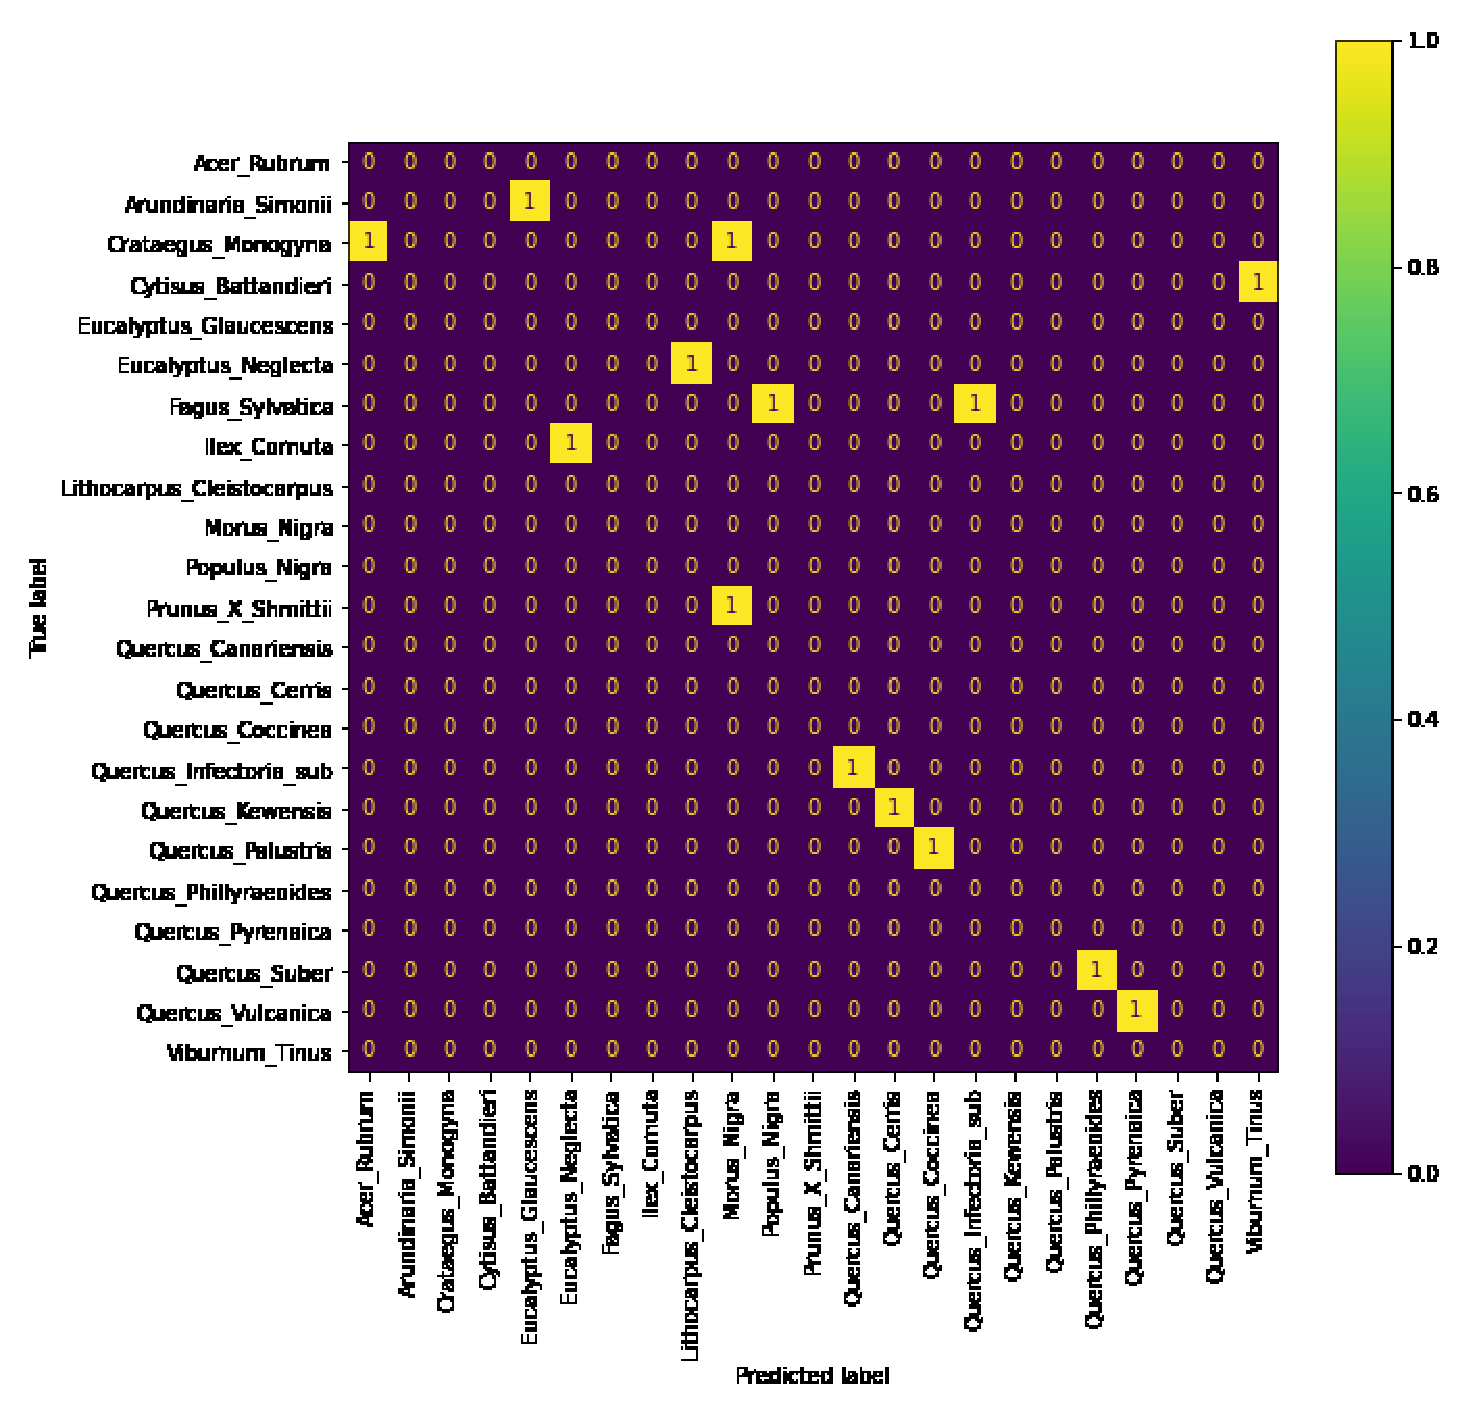
\includegraphics[scale=0.55]{images/knn_matrice_confusion} 
\par\end{centering}
\caption{\label{fig:KNN-matrice-confusion}Matrice de confusion des erreurs
commises par le KNN}
\end{figure}
\par\end{center}

\paragraph*{Conclusion}

Le classifieur KNN est optimal lorsqu'on utilise 4 voisins, la distance
de manhattan et une pondération des voisins selon la distance. Avec
ces hyperparamètres, le modèle performe très bien (> 95\% pour chaque
métrique d'évaluation) et ne semble donc ni sous-apprendre ni sur-apprendre.

\pagebreak

\subsection{Régression logistique}

Le deuxième modèle que nous avons choisi d’utiliser est le modèle
de régression logistique. Il s’agit une technique de modélisation
statistique utilisée normalement pour prédire la probabilité d'appartenance
à une classe binaire en fonction de variables indépendantes. Elle
est couramment utilisée dans les problèmes de classification, tels
que la prédiction de la catégorie d'appartenance d'un élément parmi
deux classes distinctes. 

Cependant, notre problème comporte plus de deux classes, mais il est
possible d’utiliser des approches adaptant la régression logistique
à un modèle multi-classes. On peut en effet utiliser une approche
dite "one-vs-rest" (OvR) ou multinomiale. Ces 2 approches sont disponibles
via le paramètre multi\_class de sklearn.LogisticRegression. La différence
principale entre ces 2 méthodes est qu’en OvR, un modèle de régression
est créé pour chaque classe par rapport aux autres classes combinées
alors qu’avec la méthode multinomiale, toutes les classes sont gérées
en même temps. Dans le cadre du modèle que nous avons créé, après
avoir fait des tests de performances en changeant seulement la valeur
du paramètre multi\_class, nous n’avons pas observé de différences
remarquables de performances, nous avons donc laissé le paramètre
en automatique, soit en OvR. 

Les hyperparamètres que nous avons choisit d’optimiser sont les suivants
: 
\begin{itemize}
\item La régularisation, contrôlée par le paramètre C. Plus la valeur de
C est petite, plus la régularisation est forte. 
\item Le choix de la norme de pénalité, régulée par le paramètre penalty,
qui peut être "l1" (Lasso) ou "l2" (Ridge). 
\item Le type de solveur utilisé pour l'optimisation, spécifié par le paramètre
solver, il peut être de type ‘liblinear’, ‘newton-cg’, ‘sag’ ou ‘saga’.
Il détermine l’algorithme utilisé pour le problème d’optimisation
du modèle. 
\end{itemize}
Pour le type de solveur et la norme de pénalité, nous avons fait le
choix de tous les tester dans la recherche d’hyperparamètres de notre
modèle. Par contre, pour la régularisation, il s’agit d’une valeur
numérique , qui peut prendre n’importe quelle valeur positive, il
a donc fallu faire un choix sur la plage de données à tester. La détermination
de cette plage s’est faite par tâtonnements, en testant différentes
valeurs de C pour la recherche d’hyperparamètres. Nous avons commencé
par des valeurs proches de 10, pour arriver à obtenir des scores de
performances satisfaisants aux alentour de C = 100. Au final, la plage
de valeur testée est {[}60 ; 160{]}, avec un écart de 20 entre chaque
valeur. Nous avons choisi de nous limiter le nombre de valeurs testées
et leur amplitude afin d’avoir des temps de calculs raisonnables.\\
 

Après avoir effectué la recherche des meilleurs hyperparamètres, la
meilleure combinaison pour l’entraînement obtenue est la suivante
: C = 160, penalty = ‘l2’ et solver = ‘liblinear’, avec un score de
précision de 0.912.

Dans un premier temps, on remarque que la valeur de C est la plus
élevée parmi celles présentes dans l’intervalle de recherche. Cela
confirme les observations faites précédemment lors du processus de
recherche des valeurs des hyperparamètres à tester. Sachant que C
est l’inverse de la force de régularisation, cela signifie que moins
la régularisation est forte, mieux notre modèle performe sur les données
d’entraînement. Afin de constater l’importance de cet hyperparamètre
par rapport aux autres, nous traçons les courbes représentant les
différentes combinaisons d’hyperparamètres testés : 
\begin{figure}[h]
\centering{}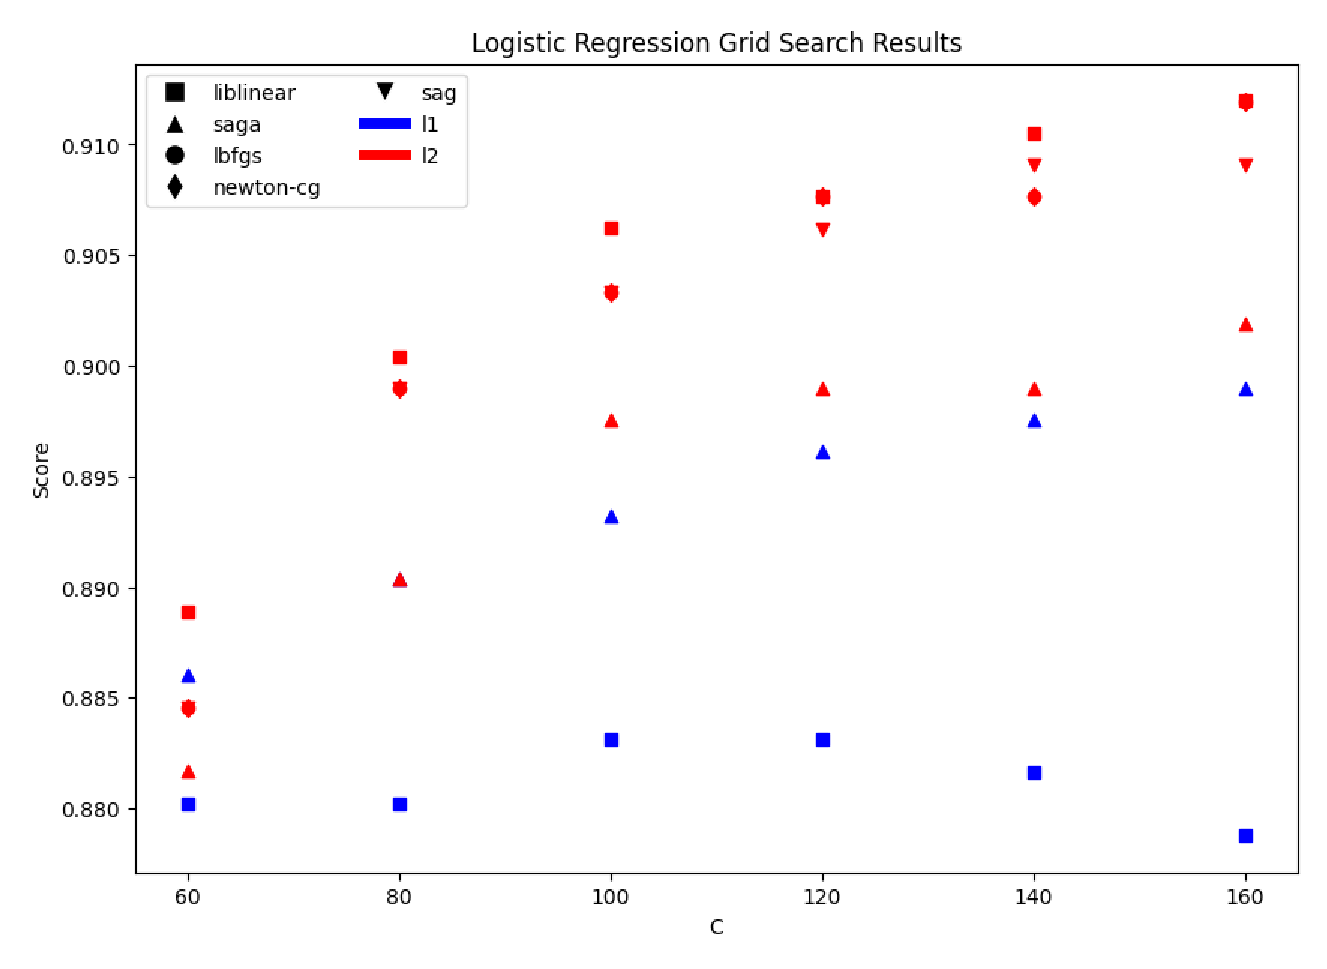
\includegraphics[width=0.7\linewidth]{images/courbe_lr}
\caption{Courbe de score du modèle Logistic Regression pour différents hyperparamètres}
\end{figure}

Dans un premier temps, il est important de noter que toutes les combinaisons
possibles d’hyperparamètres ne sont pas présentes. Cela est dû au
fait que certains solvers ne sont compatibles qu’avec certaines pénalités,
comme newton-cg qui n’est compatible qu’avec une pénalité l2. 

Ensuite, nous observons clairement une augmentation nette du score
plus la valeur de C est élevée, pour toutes les combinaisons d’hyperparamètres,
hormis quand le solver est liblinear et la pénalité l1. En outre,
le choix de la pénalité a également un impact important sur les performances,
les courbes en rouges, représentant la pénalité l2 sont au-dessus
des bleues représentant l1. Cela peut s’expliquer par plusieurs raisons.
La pénalité l2 est meilleure lorsque les données possèdent des caractéristiques
corrélées, ce qui est le cas pour nos données où les 3 caractéristiques
sont divisées en 64 sous caractéristiques. De plus , la pénalité l2
est souvent utilisée dans les cas où le nombre d’observations est
limité comparé au nombre de classes, correspondant bien à notre jeu
de données. 

Enfin, pour les solvers couplés à la pénalité l2, nous observons que
liblinear, lbfgs, sag et newton-cg obtiennent des résultats assez
similaires, et avec saga légèrement en-dessous. Le solver liblinear
reste tout de même le plus performant peut importe la valeur de C,
mais avec une marge de moins en moins grande plus C augmente. Pour
notre modèle, le choix du solver n’a donc pas d’impact significatif
sur les performances par rapport aux deux autres hyperparamètres. 

Pour réellement mesurer les performances du meilleur modèle sur l’ensemble
d’entraînement, nous l’évaluons sur un ensemble de test composé de
données que le modèle n’a jamais rencontré. Voici les valeurs moyennes
des métriques de performances obtenues pour chaque classe : 
\begin{itemize}
\item Précision : 93,822 \textpm{} 14,766 \%
\item Rappel : 92,929 \textpm{} 16,682 \%
\item F1-score : 92,350 \textpm{} 13,945 \% 
\end{itemize}
Nous traçons également les boxplots correspondants : 
\begin{figure}[h]
\centering{}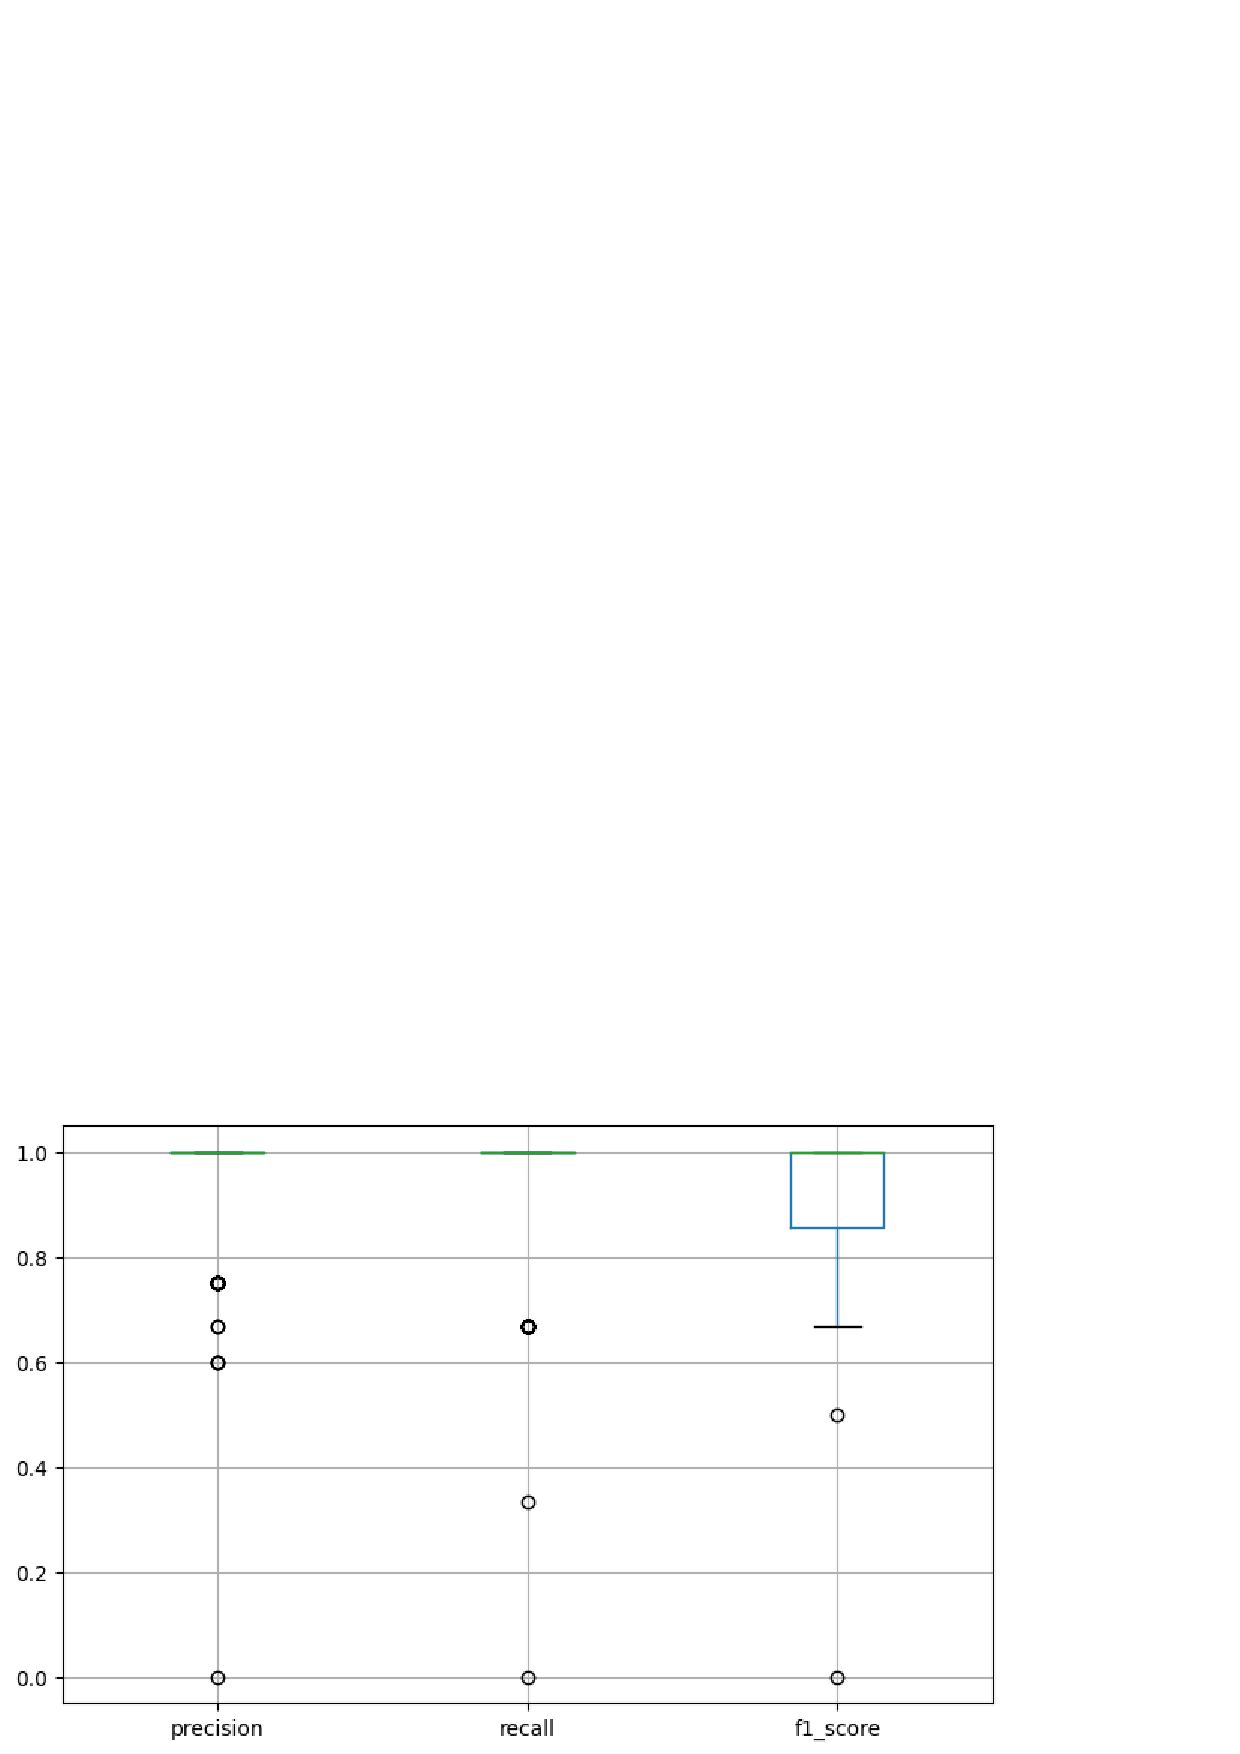
\includegraphics[width=0.7\linewidth]{images/boxplot_lr}
\caption{Distribution des métriques d’évaluation pour le modèle Logistic Regression}
\end{figure}

D’abord, on remarque que les valeurs des 3 métriques de performances
sont très élevées, avec 93,8\% de précision et un rappel et f1-score
aux alentours de 92,3\%. Comme on peut le voir dans les boxplots,
les prédictions sont correctes pour la grande majorité des classes,
avec seulement très peu de valeurs aberrantes (outliers). On peut
cependant observer que le boxplot du f1-score est un peu plus étendu,
indiquant quelques erreurs de prédictions, mais rien de critique,
la médiane étant aux alentours de 0.9. 

Il existe cependant des classes pour lesquelles le modèle a moins
bien performé. Au total, 34 classes sur les 99 on un f1-score non
parfait, c’est-à-dire différent de 1. Cela n’est absolument pas alarmant
sur les performances de notre modèle, mais indique que des points
d’améliorations subsistent pour encore augmenter les performances
de celui-ci. 

Enfin, nous dressons la matrice de confusion qui montre toutes les
erreurs de prédictions, en affichant les couples de classes où une
classe prédite était différente de la classe réelle, avec le nombre
d’occurrences.

\begin{figure}[h]
\centering{}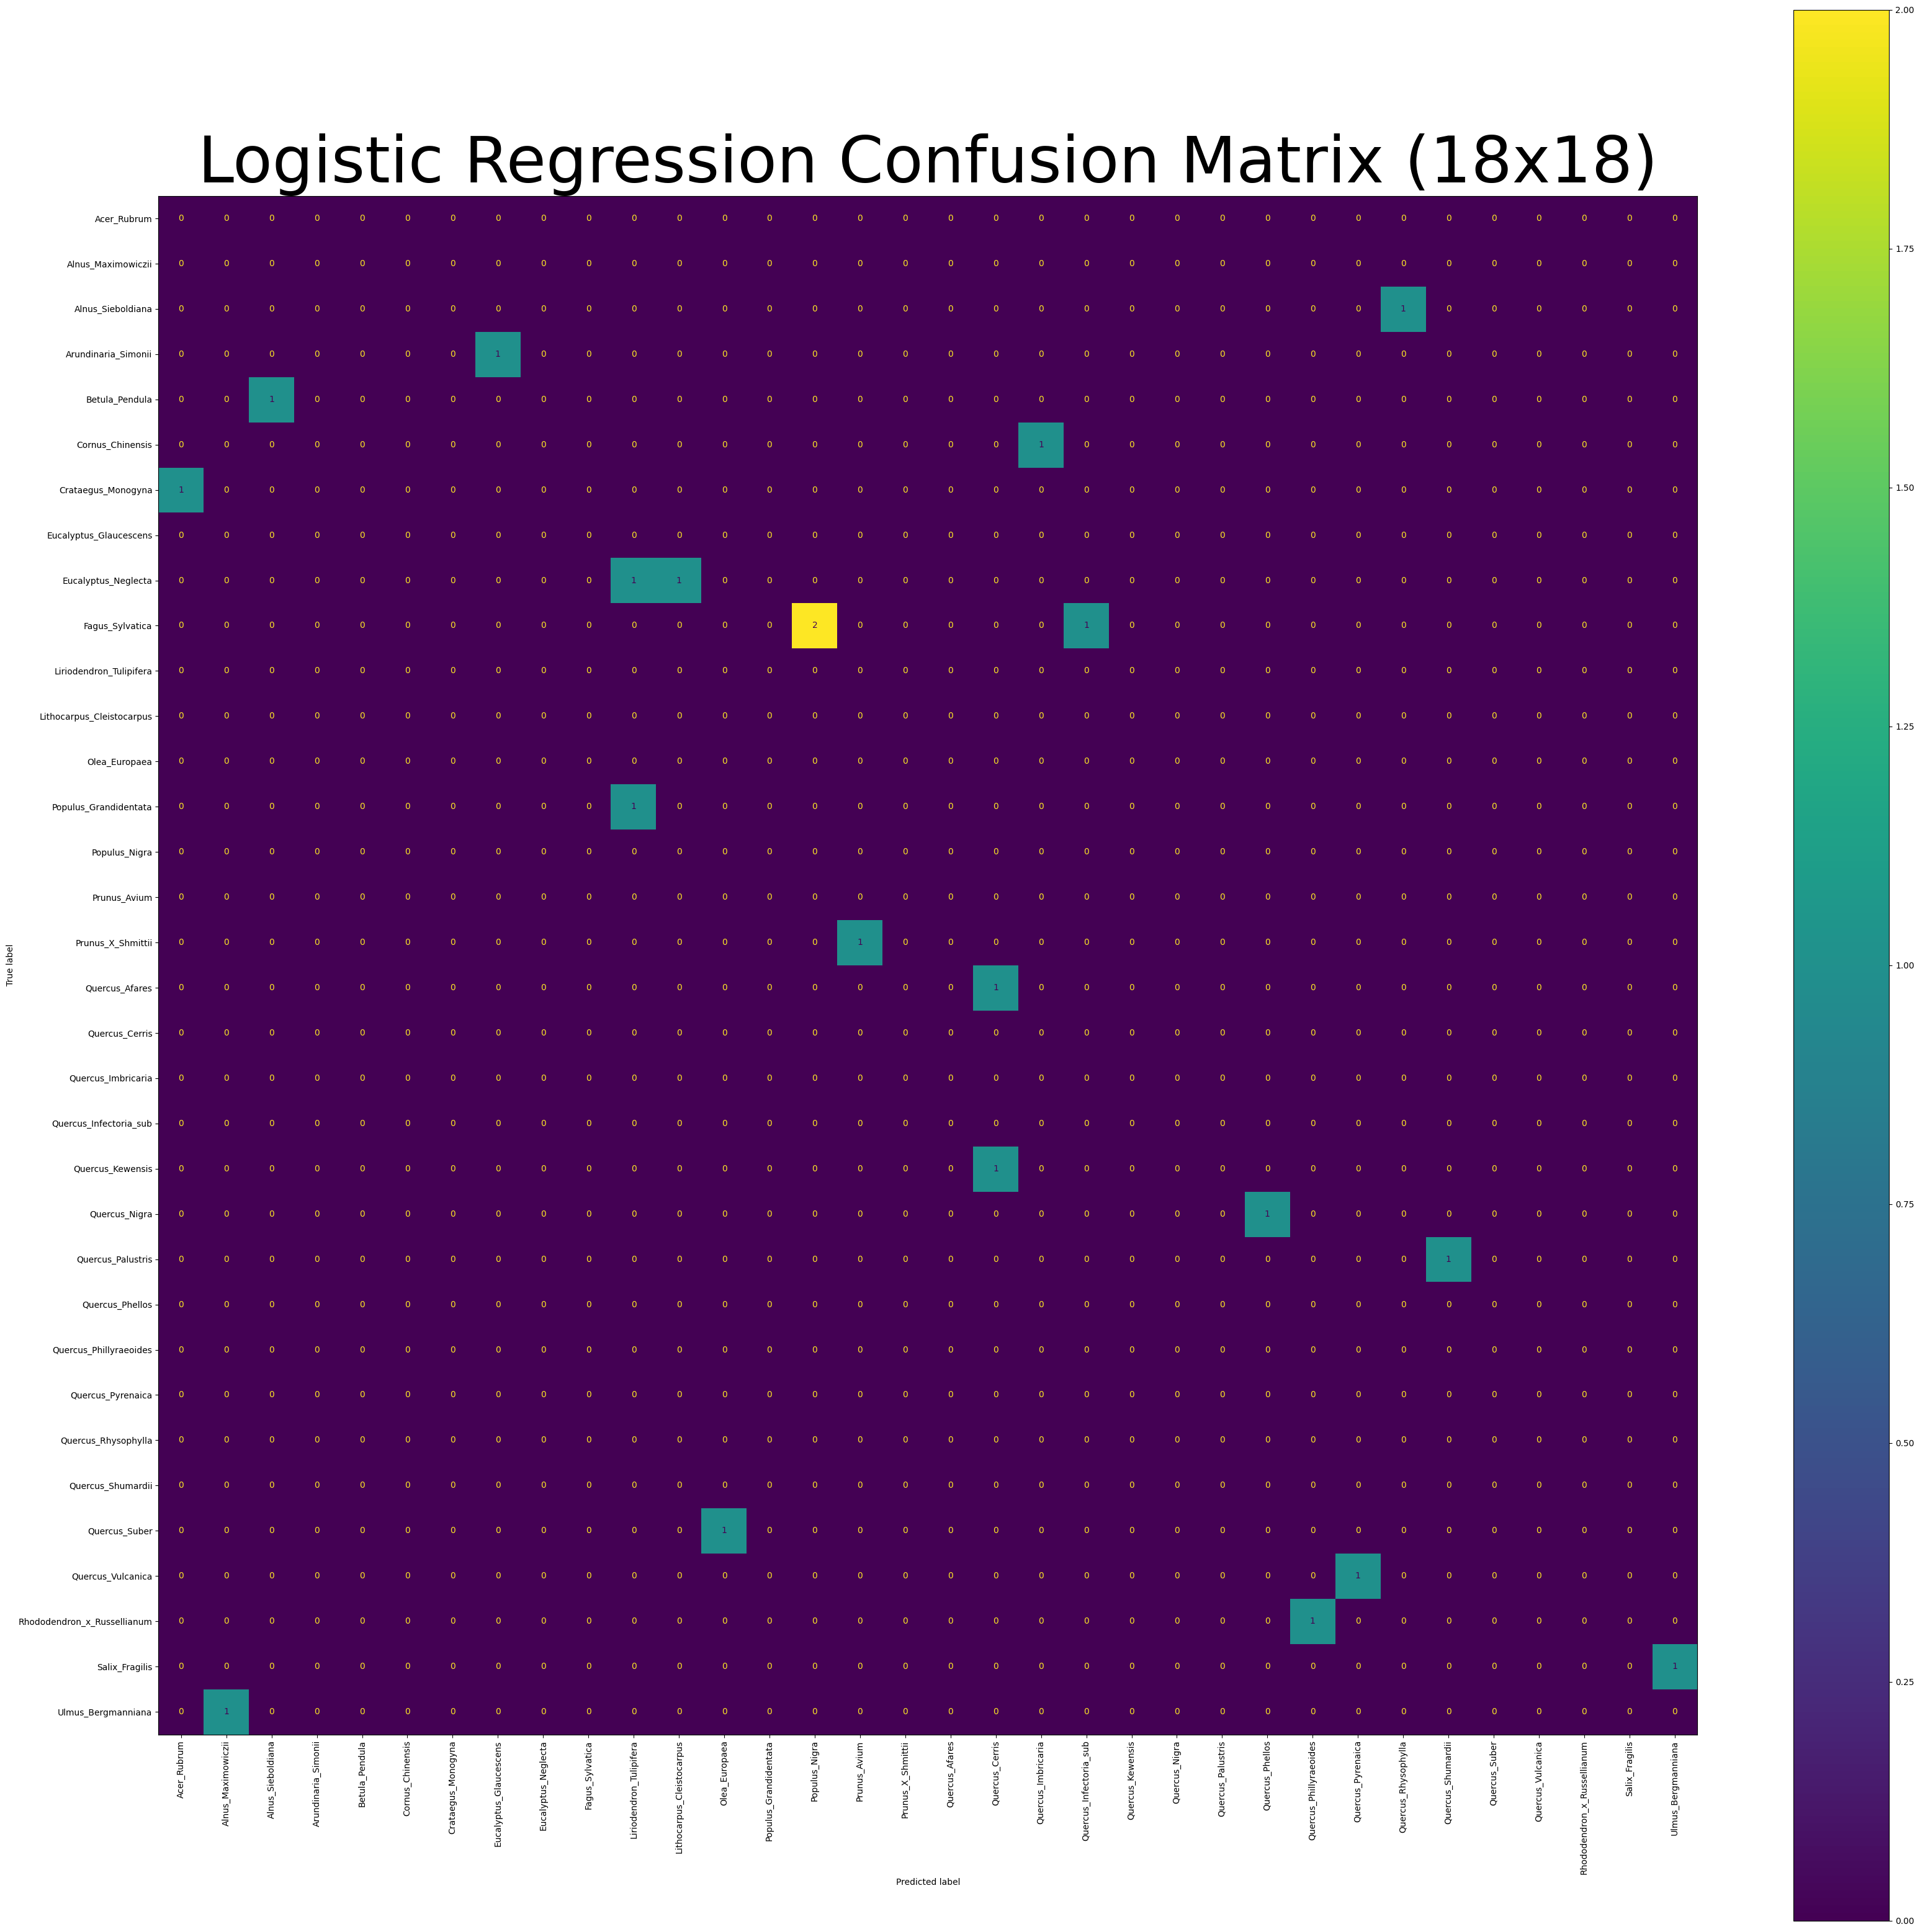
\includegraphics[width=0.7\linewidth]{images/matrix_lr}
\caption{Matrice de confusion du modèle Logistic Regression}
\end{figure}

Comme observé précédemment via les métriques de performances, nous
voyons que les erreurs de prédictions sont rares et ne sont pas concentrées
sur une classe en particulier. On peut seulement relever le fait que
la feuille de type Falgus\_Sylvatica est la seule classe a mal avoir
été prédite à 3 reprises.\\[2\baselineskip]

\paragraph*{Conclusion}

Malgré son origine binaire, le modèle de régression logistique s’est
révélé plutôt performant pour résoudre notre problème de classification.
Nous avons en ce sens adapté la régression logistique à un modèle
multi-classes en utilisant l'approche OvR.

Les meilleurs hyperparamètres trouvés sont la régularisation C = 160,
la norme de pénalité = 'l2'et le type de solveur 'liblinear', avec
un score de précision de 91,2\% sur les données d’entraînement, et
des métriques de performance allant de 92 à 94\% sur les données de
test.

L'analyse des performances en fonction de la régularisation (C) a
révélé que des valeurs plus élevées de C ( donc moins de régularisation)
ont conduit à de meilleures performances sur l'ensemble d'entraînement.
La pénalité l2 a également montré des performances supérieures à la
pénalité l1, probablement en raison de la nature de nos données avec
des caractéristiques corrélées. Enfin, le choix du solveur n’a pas
eu d’impact significatif sur les performances, particulièrement pour
des valeurs de C élevées.

Les boxplots ont montré une bonne cohérence des performances avec
peu de valeurs aberrantes et a matrice de confusion a identifié quelques
erreurs de prédictions, mais dans l'ensemble, le modèle a bien généralisé
sur l'ensemble des classes. Il y a des opportunités d'amélioration
spécifiques pour certaines classes où le modèle a rencontré plus de
difficultés.

En conclusion, la régression logistique s'est révélée être une approche
robuste pour notre problème de classification de feuilles à 99 classes,
offrant de bonnes performances sur l'ensemble de test. Des ajustements
futurs pourraient inclure des stratégies spécifiques pour les classes
présentant des difficultés, ainsi que l'optimisation plus poussée
d’autres hyperparamètres en acceptant des temps de calculs plus élevés,
pour une comparaison approfondie des performances avec le modèle actuel.

\pagebreak

\subsection{Machine à vecteurs de support}

Notre troisième classifieur est la machine à vecteur de support. L'avantage
de ce classifieur, c'est qu'il performe normalement très bien avec
des données qui ont beaucoup de dimensions, ce qui est notre cas.
On s'attend donc à de bon résultat.

Les hyperparamètres du SVM sont les suivants : 
\begin{itemize}
\item Un paramètre de régularisation (\texttt{C}) : plus il est grand, moins
la régularisation est forte 
\item Le noyau : linéaire, gaussien, polynomial ou sigmoidal 
\item Un paramètre gamma utilisé par les noyaux gaussien, polynomial et
sigmoidal : soit \textit{scale}, soit \textit{auto} 
\end{itemize}
L'hyperparamètre le plus important est évidemment le noyau. C'est
le noyau qui détermine quelle genre de fonction le SVM pourra apprendre.
On veut donc tester le plus de noyau possible pour être sûr de trouver
le bon.

Cependant, lorsqu'on utilise un noyau polynomial, on a un hyperparamètre
supplémentaire : le degré. Comme rechercher le degré optimal en même
temps que les autres hyperparamètres prendrait trop de temps, on l'a
fait séparément et on a trouvé que le degré optimal est de 1.

Les meilleurs hyperparamètres pour notre ensemble d'entrainement sont
: 
\begin{itemize}
\item Régularisation : 6,0 
\item Noyau : polynomial de degré 1 
\item Gamma : \textit{scale} 
\end{itemize}
La figure \ref{fig:Score-du-SVM} montre les résultats de l'entrainement
pour les différentes valeurs d'hyperparamètres. On voit bien que le
type de noyau a un impact significatif sur les performances du modèle.
Le noyau linéaire est le moins performant, ce qui est normal si on
suppose que les données ne sont pas linéairement séparable. Les noyaux
polynomial, gaussien et sigmoidal sont très similaires, mais le noyau
sigmoidal est toujours moins performant.

On remarque aussi que les performances du modèle atteignent un plateau
à \texttt{C=2}. Au-delà de cette valeur, la différence de performance
entre le noyau polynomial et le noyau gaussien n'est pas significative.
Nous choisirons quand même le noyau polynomial pour la suite des tests.

Finalement, le paramètre gamma ne semble pas avoir d'influence sur
les performances. Lorsque gamma est à \textit{auto}, le modèle est
toujours mauvais. 
\begin{center}
\begin{figure}[h]
\begin{centering}
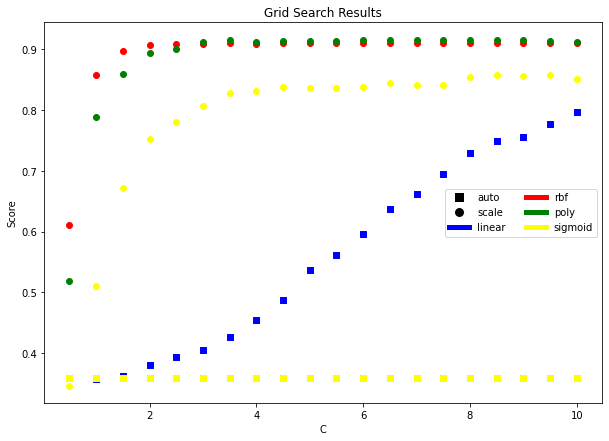
\includegraphics[scale=0.55]{images/svm_cross_validation} 
\par\end{centering}
\caption{\label{fig:Score-du-SVM}Score du SVM selon les différents hyperparamètres}
\end{figure}
\par\end{center}

Nous avons testé le modèle avec les hyperparamètres optimaux sur l'ensemble
de test. Pour chacune des métriques d'évaluation, voici la moyenne
calculée pour l'ensemble des classes : 
\begin{itemize}
\item Précision : 95,522 \textpm{} 10,962 \% 
\item Rappel : 93,603 \textpm{} 15,560 \% 
\item F1-score : 93,271 \textpm{} 11,723 \% 
\end{itemize}
\begin{center}
\begin{figure}[h]
\begin{centering}
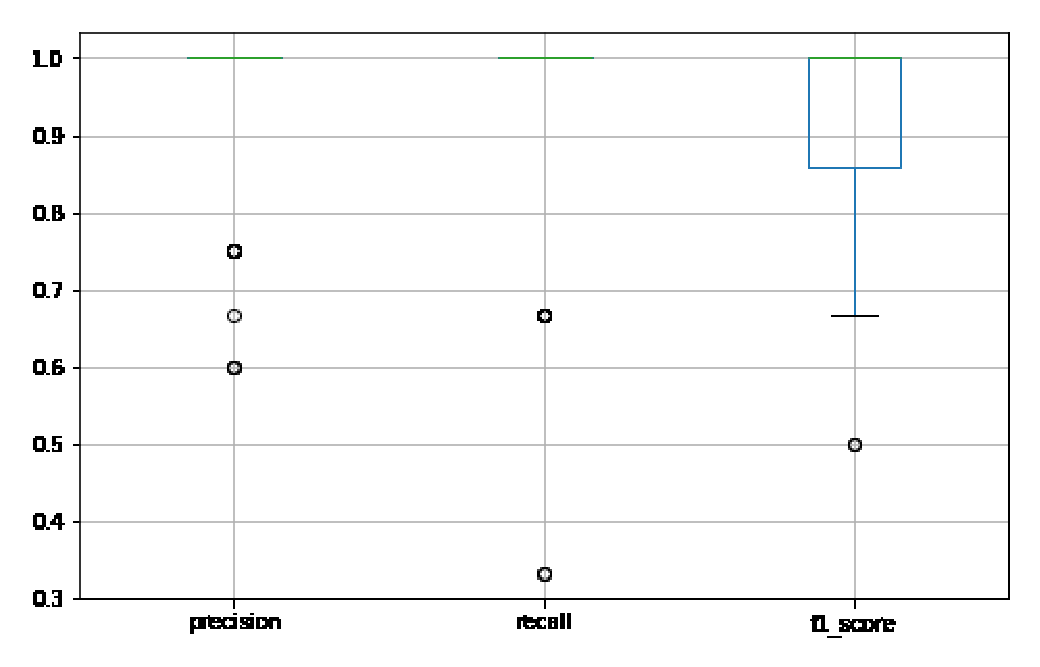
\includegraphics[scale=0.6]{images/svm_evaluation} 
\par\end{centering}
\caption{\label{fig:SVM-evaluation}Distribution des métriques d'évaluation
pour le SVM}
\end{figure}
\par\end{center}

La figure \ref{fig:SVM-evaluation} montre la distribution des classes
pour chaque métrique. Encore une fois, les prédictions sont parfaites
(métrique à 1,0) pour la grande majorité des classes. Si on regarde
la matrice de confusion des erreurs commises, figure \ref{fig:SVM-matrice-confusion},
on ne remarque aucune relation particulière. Les erreurs sont réparties
assez uniformément parmi les différentes classes. 
\begin{center}
\begin{figure}[H]
\begin{centering}
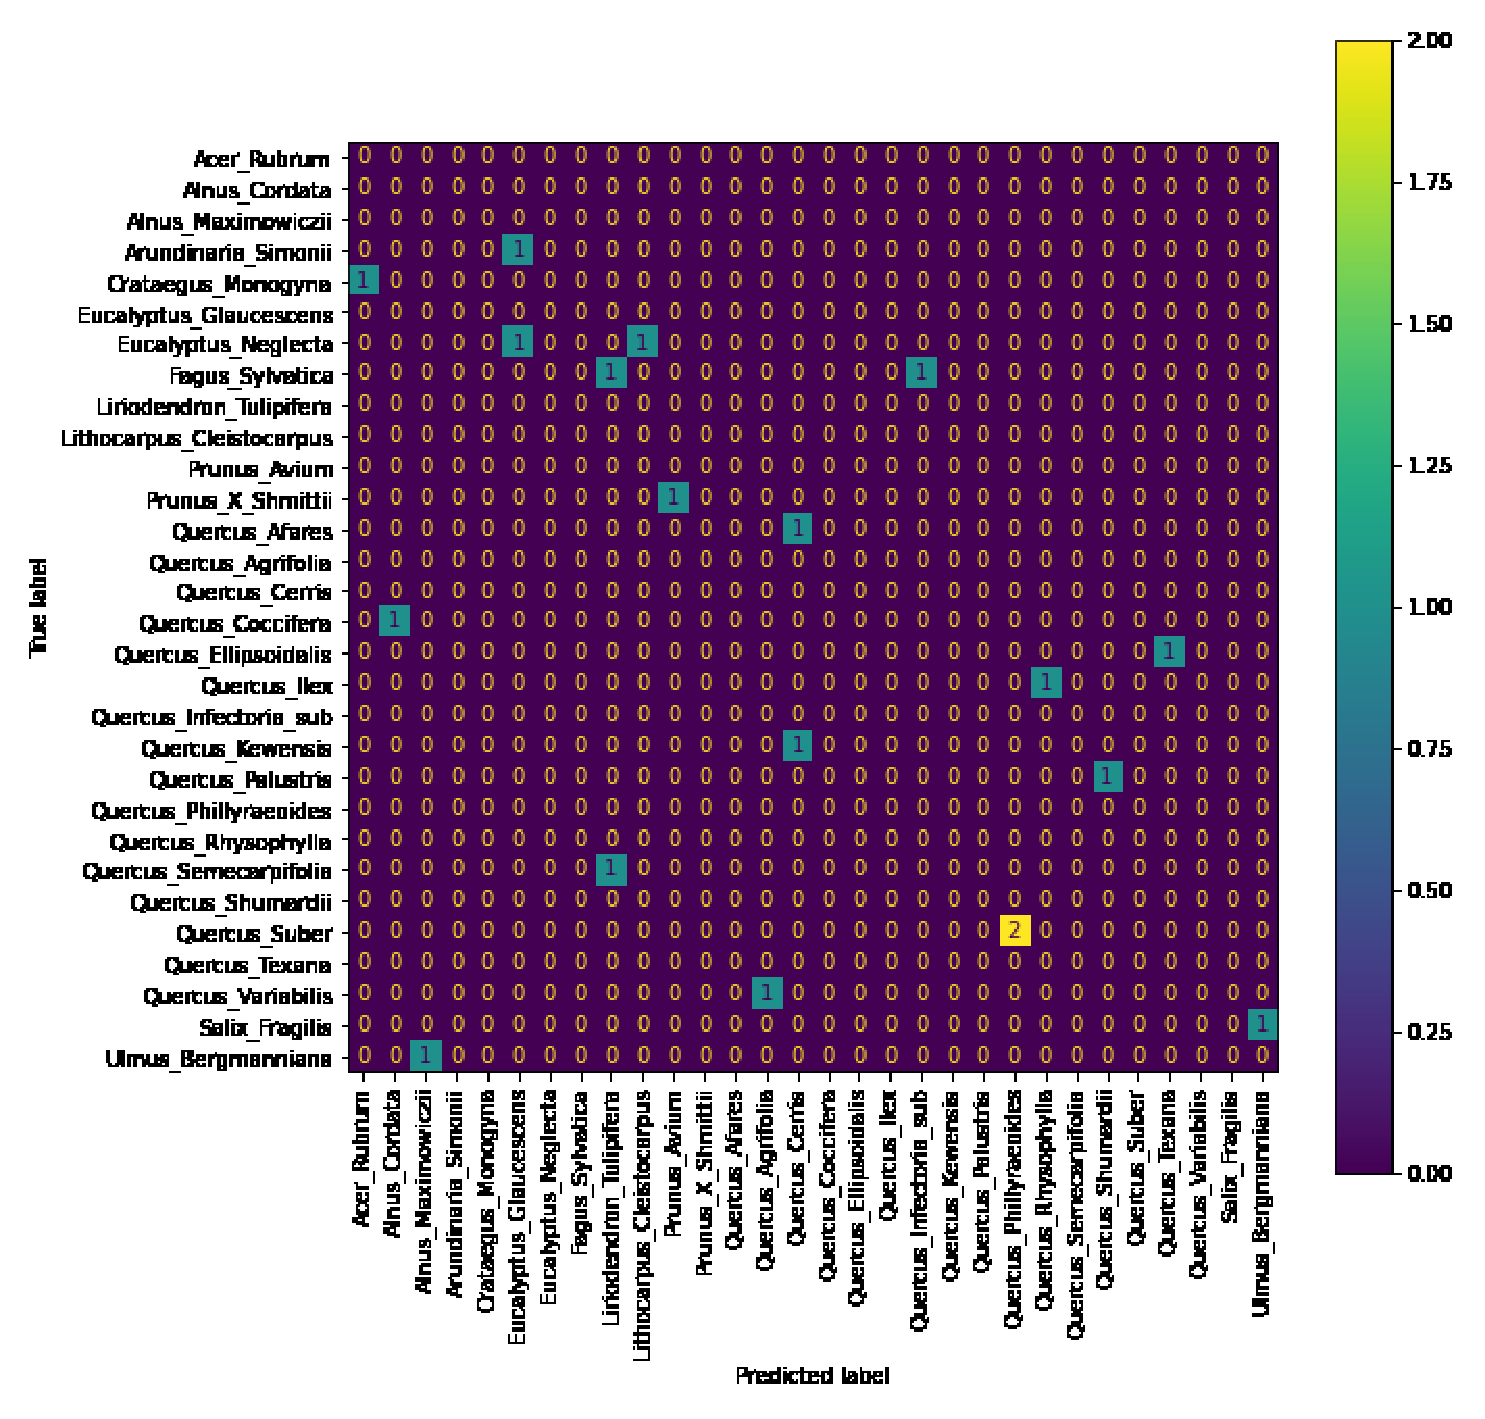
\includegraphics[scale=0.5]{images/svm_matrice_confusion} 
\par\end{centering}
\caption{\label{fig:SVM-matrice-confusion}Matrice de confusion des erreurs
commises par le SVM}
\end{figure}
\par\end{center}

\paragraph*{Conclusion}

Le classifieur SVM est optimal lorsqu'on utilise un noyau polynomial
de degré 1 avec un paramètre de régularisation de 6. Cependant, un
noyau gaussien avec le même paramètre de régularisation a des performances
presque identique. On ne peut donc pas vraiment dire si l'un est meilleur
que l'autre. Avec ces hyperparamètres, le SVM performe très bien et
ne semble ni sur-apprendre ni sous-apprendre.

\pagebreak

\subsection{Classifieur AdaBoost}

Le quatrième classifieur que nous avons sélectionné pour évaluation
est l'Adaboost. Il s'agit d'un modèle qui combine plusieurs classifieurs
faibles pour former un ensemble robuste et performant. L'Adaboost
accorde des poids différents aux données d'entrainement, mettant davantage
l'accent sur celles qui ont été mal classées par les classifieurs
précédents. Cela en fait un modèle adaptatif et capable de s'ajuster
aux erreurs précédentes.

L'avantage de l'Adaboost réside dans sa capacité à s'adapter à des
ensembles de données complexes sans nécessiter beaucoup d'ajustements
d'hyperparamètres. Cependant, il peut être sensible au bruit dans
les données et à des valeurs aberrantes.

Dans notre contexte, nous anticipons des performances prometteuses
avec l'Adaboost, car il est bien adapté à la classification de feuilles.
Nous supposons que les caractéristiques distinctives des différentes
espèces de feuilles seront correctement exploitées par l'Adaboost,
conduisant ainsi à des prédictions précises et discriminantes

Les hyperparamètres de l'Adaboost sont les suivants : 
\begin{itemize}
\item Le nombre d'estimateurs 
\item Le learning rate 
\item Le type d'estimateur ou classifieur faible 
\end{itemize}
Les hyperparamètres les plus importants est évidemment le type d'estimateur
et; c'est lui qui détermine vraiment la capacité du modèle.

Les meilleurs hyperparamètres pour notre ensemble d'entrainement sont
: 
\begin{itemize}
\item Le nombre d'estimateurs: 64 
\item Le learning rate: 0,01 
\item Le type d'estimateur ou classifieur faible: ExtraTreesClassifier 
\end{itemize}
La figure \ref{fig:Score-adaboost} montre les résultats de l'entrainement
pour les différentes valeurs d'hyperparamètres. On remarque une différence
significative entre le classifieur SVM (qui n'a pas été tracé due
à ses pauvres performances) et les deux autres.
\begin{center}
\begin{figure}[h]
\begin{centering}
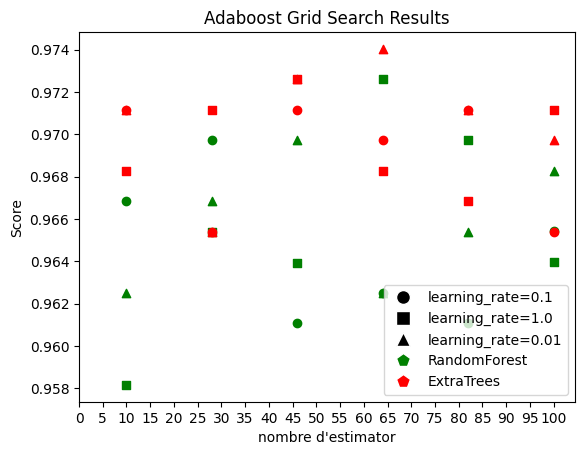
\includegraphics[scale=0.55]{images/adaboost_boxplot} 
\par\end{centering}
\caption{\label{fig:Score-adaboost}Score de l'adaboost selon les différents
hyperparamètres}
\end{figure}
\par\end{center}

On peut voir sur le graphique que le score est différent en fonction
du type d'estimateur et que learning rate n'influe pas grandement
le résultat. Le nombre d'estimateur influence légérement les résultats.

Nous avons évalué les performances du modèle sur l'ensemble de test
en utilisant les hyperparamètres optimaux. Pour chaque métrique d'évaluation,
la moyenne a été calculée en considérant l'ensemble des classes : 
\begin{itemize}
\item Précision : 97,593 \textpm{} 8,368 \% 
\item Rappel : 96,633 \textpm{} 11,163 \% 
\item F1-score : 96,518 \textpm{} 8,737 \% 
\end{itemize}
\begin{center}
\begin{figure}[h]
\begin{centering}
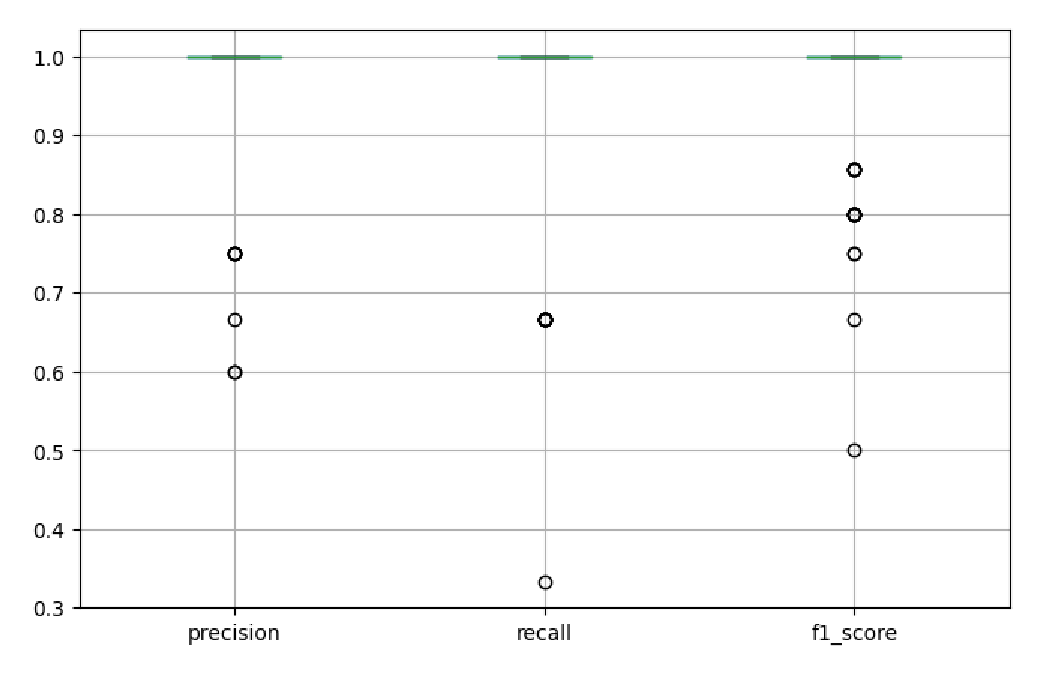
\includegraphics[scale=0.5]{images/adaboost_evaluation} 
\par\end{centering}
\caption{\label{fig:adaboost-evaluation}Distribution des métriques d'évaluation
pour l'adaboost}
\end{figure}
\par\end{center}

La figure \ref{fig:adaboost-evaluation} montre la distribution des
classes pour chaque métrique. Étant donné le nombre élevé de classes
(99), l'évaluation des performances pour chaque classe individuelle
peut rapidement devenir impraticable. Pour obtenir une vue d'ensemble,
nous analysons plutôt la moyenne des métriques à travers l'ensemble
des classes. Globalement, notre modèle démontre une performance robuste,
manifestant à la fois une précision et une justesse élevées.

Comme on peut le voir dans le boxplot, les prédictions sont parfaites
(métriques à 1.0) pour la grande majorité des classes.

La figure \ref{fig:adaboost-matrice-confusion} montre une matrice
de confusion des classes pour lesquelles le modèle a commis des erreurs.
On ne remarque aucune relation parmi les erreurs commises. Il s'agit
donc probablement de données pour lesquelles les caractéristiques
sont moins distinctes. 
\begin{center}
\begin{figure}[h]
\begin{centering}
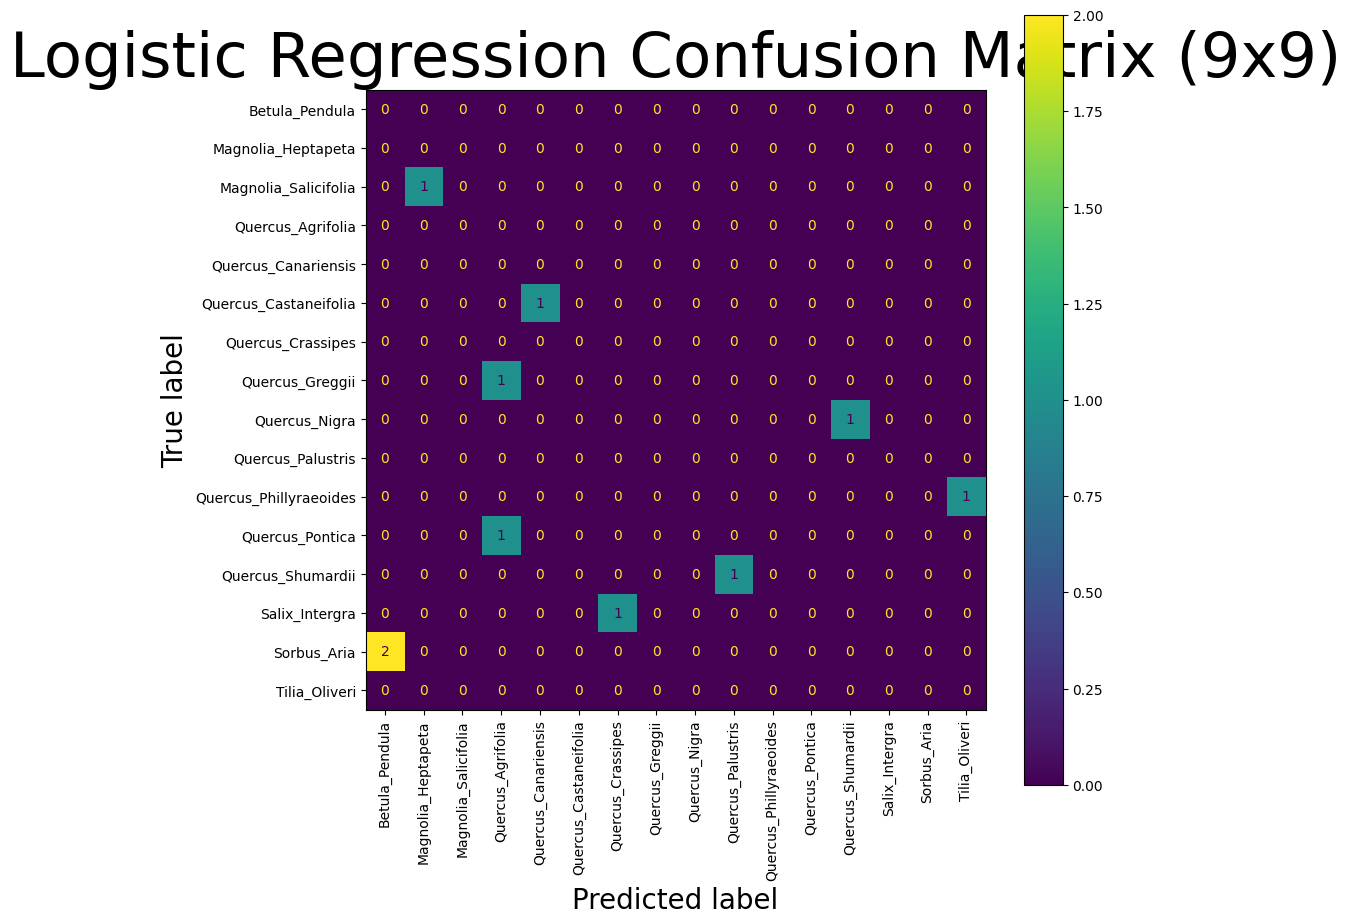
\includegraphics[scale=0.45]{images/adaboost_matrice_confusion} 
\par\end{centering}
\caption{\label{fig:adaboost-matrice-confusion}Matrice de confusion des erreurs
commises par l'adaboost}
\end{figure}
\par\end{center}

\paragraph*{Conclusion}

Le classifieur adaboost est optimal lorsqu'on utilise un grand nombre
d'estimateurs, et des classifieurs faibles adéquat. Avec ces hyperparamètres,
le modèle performe très bien (> 96.5\% pour chaque métrique d'évaluation)
et ne semble donc ni sous-apprendre ni sur-apprendre.

\pagebreak

\subsection{Arbre de décisions}

Le cinquième modèle que nous avons choisi d’utiliser est l'arbre de
décision. Il s'agit d'une méthode de modélisation qui prend des décisions
selon une structure arborescente. Les arbres de décision sont conçus
pour résoudre des problèmes de classification avec plusieurs classes,
comme dans notre cas. Cette approche est particulièrement adaptée
pour diviser l'espace des caractéristiques en régions, en prenant
des décisions basées sur des seuils dans les caractéristiques. Les
arbres de décision sont largement utilisés dans la classification
en raison de leur capacité à capturer des relations complexes entre
les caractéristiques et la classe cible. 

Les hyperparamètres que nous avons choisi d’optimiser sont les suivants
: - La profondeur maximale de l'arbre (max\_depth). Chaque niveau
de profondeur correspond à une séparation supplémentaire des données
en sous-groupes. Une profondeur à None indique qu'il n'y a pas de
restriction sur celle-ci. 
\begin{itemize}
\item Le nombre minimal d'échantillons requis dans un nœud pour qu’il soit
divisé (min\_samples\_split). 
\item Le critère de qualité de la division (criterion), qui peut être ‘gini’,
‘entropy’ ou ‘log\_loss’. 
\item La stratégie de division aux noeuds (splitter), qui peut être ‘best’
ou ‘random’. 
\end{itemize}
Bien que la profondeur maximale soit souvent l'hyperparamètre le plus
crucial dans les arbres de décisions, nous explorons également l'impact
des autres hyperparamètres sur les performances du modèle. 

Pour le critère de qualité, nous avons fait le choix de tester les
3 types disponibles, avec ‘gini’ qui se base sur la mesure d’impureté
des classes dans un nœud, ‘entropy’ qui mesure l’information contenue
dans un nœud et ‘log\_loss’ qui calcule des pertes logarithmiques.
De même pour la stratégie de division aux nœuds : le splitter de type
‘best’ choisit la division qui maximise la mesure définie par le critère
de qualité choisi, alors que ‘random’ choisi une division parmi un
ensemble aléatoire de divisions possibles, sans forcément évaluer
toutes les possibilités. 

Concernant la profondeur maximale de l’arbre, nous avons procédé comme
pour d’autres modèles, où nous avons effectué des tests à tâtons pour
observer quelles plages de valeurs seraient intéressantes à tester
lors de la recherche d’hyperparamètres. Après quelques essais, les
valeurs intéressantes semblent se trouver à partir d’une profondeur
proche de la centaine, allant jusqu’au millier. Également, nous avons
intégré la profondeur ‘None’, indiquant une non-restriction sur la
profondeur. 

Pour le min\_samples\_split, nous avons procédé de même, en remarquant
que les valeurs revenant le plus souvent dans les meilleurs modèles
étaient soit 2 ou 5. 

Après avoir effectué la recherche des meilleurs hyperparamètres, la
meilleure combinaison pour l’entraînement obtenue est la suivante
: max\_depth = None, min\_samples\_split = 5 et criterion = ‘gini’
et splitter = ‘random’ avec un score de précision de 0,615. 

Pour la profondeur maximale des arbres, on constate que l'absence
de limite de profondeur (None) semble donc être préférable. Cela suggère
que permettre aux arbres de se développer sans restriction de profondeur
donne de meilleurs résultats dans ce contexte. Il est important de
rappeler qu’il ne s’agit que des données d’entraînement, donc il est
assez normal qu’avec cette liberté au niveau de la profondeur, le
modèle s’ajuste le mieux aux données d’entraînement. De plus, cela
fait d’autant plus sens au vu de la grande quantité de classes que
notre jeu de données possède. 

On peut examiner les performances du modèle en considérant le score
associé à cette limite de profondeur et évaluer l'influence des autres
hyperparamètres sur ces résultats : 
\begin{figure}[h]
\centering{}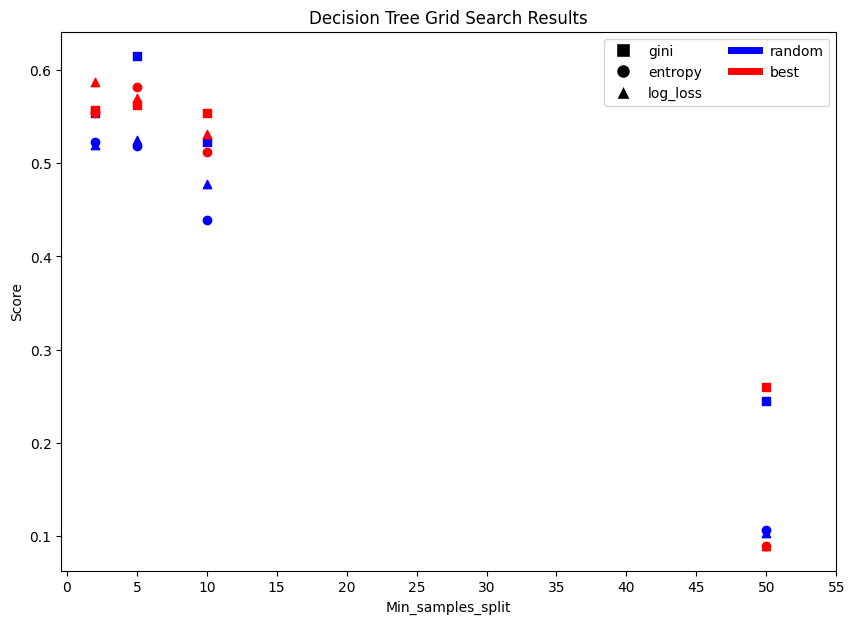
\includegraphics[width=0.7\linewidth]{images/courbe_dt}
\caption{Courbe de score du modèle Decision Tree pour différents hyperparamètres}
\end{figure}

D’abord, nous pouvons rapidement observer que plus le nombre minimal
d'échantillons requis dans un nœud pour qu’il soit divisé augmente,
moins le modèle est performant. Il est assez simple d’expliquer cela,
en effet si on augmente cette valeur, le modèle est contraint de créer
des divisions dans les nœuds uniquement s'il y a un nombre relativement
élevé d'échantillons dans ces nœuds. Cela peut conduire à un arbre
de décision moins profond et plus généralisé, car les divisions ne
sont autorisées que lorsque le modèle détecte des schémas plus forts
dans les données. De plus, par rapport à notre jeu de donnée, cela
peut clairement impacter les faibles différenciations pouvant exister
entre certaines des 99 classes présentes, et donc faire chuter les
performances du modèle. 

Concernant la stratégie de division aux nœuds, la ‘best’ paraît être
la meilleure en moyenne, par rapport à la stratégie ‘random’, qui
arrive cependant parfois à obtenir de meilleurs résultats. Cela s’explique
simplement par la nature de ces stratégies : le splitter ‘best’ va
systématiquement choisir la division la plus bénéfique en termes de
critère de qualité, alors que le random va parfois être chanceux sur
ses choix de division, expliquant sa supériorité en performances par
moment, mais en moyenne ses résultats seront plus faibles. 

Enfin, nous observons que le critère de division donnant les meilleurs
résultats paraît être ‘gini’, malgré le fait que les autres critères
possèdent des performances assez proches. D’après la littérature,
le critère ‘gini’ est surtout privilégié pour alléger les temps de
calculs qu’induisent les méthodes ‘entropy’ et ‘log\_loss’. Dans notre
cas en particulier, le choix de ce paramètre ne possède d’impact important
sur les performances du modèle. 

Pour réellement mesurer les performances du meilleur modèle sur l’ensemble
d’entraînement, nous l’évaluons sur un ensemble de test composé de
données que le modèle n’a jamais rencontré. Voici les valeurs moyennes
des métriques de performances obtenues pour chaque classe : 
\begin{itemize}
\item Précision : 71,125 \textpm{} 14,766 \% 
\item Rappel : 66,33 \textpm{} 16,682 \% 
\item F1-score : 66,365 \textpm{} 13,945 \%
\end{itemize}
\begin{figure}[h]
\centering{}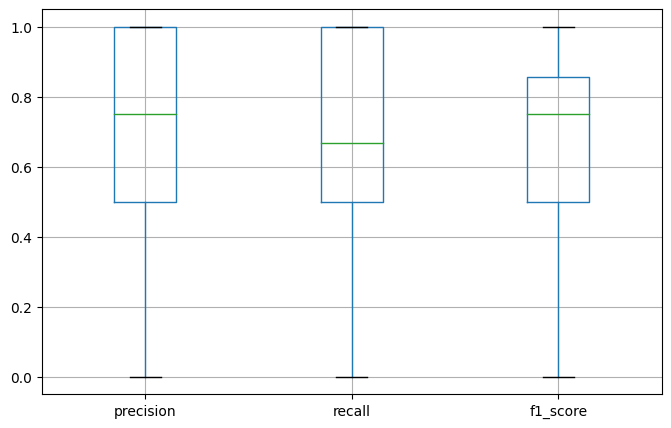
\includegraphics[width=0.7\linewidth]{images/boxplot_dt}
\caption{Distribution des métriques d’évaluation pour le modèle Decision Tree}
\end{figure}

D’abord, nous remarquons que les métriques de performances sont assez
faibles, entre 66 et 72\%, distantes de l’intervalle des $85-100\%$
qui caractérise les bonnes performances d’un modèle. Ces observations
se traduisent sur la forme des boxplots tracés, où l’écart inter-quartile
est très prononcé, de l’ordre de 0.5 pour la précision et le rappel
et 0.35 pour le f1-score, traduisant de nombreuses erreurs de prédiction.
De plus, les extrémités des boxplots s’étendent sur l’entièreté de
l’intervalle {[}0 ; 1{]}. 

Cependant, le point positif à retirer de ces résultats est que l’on
a obtenu de meilleures performances sur l’ensemble de test comparativement
aux résultats sur les données d’entraînement. 

Il existe donc beaucoup de classes pour lesquelles le modèle a moins
bien performé. Au total, 83 classes sur les 99 ont un f1-score non
parfait, c’est-à-dire différent de 1, témoignant des faibles performances
du modèle. 

Enfin, nous dressons la matrice de confusion qui montre toutes les
erreurs de prédictions, en affichant les couples de classes où une
classe prédite était différente de la classe réelle, avec le nombre
d’occurrences.

\begin{figure}[h]
\centering{}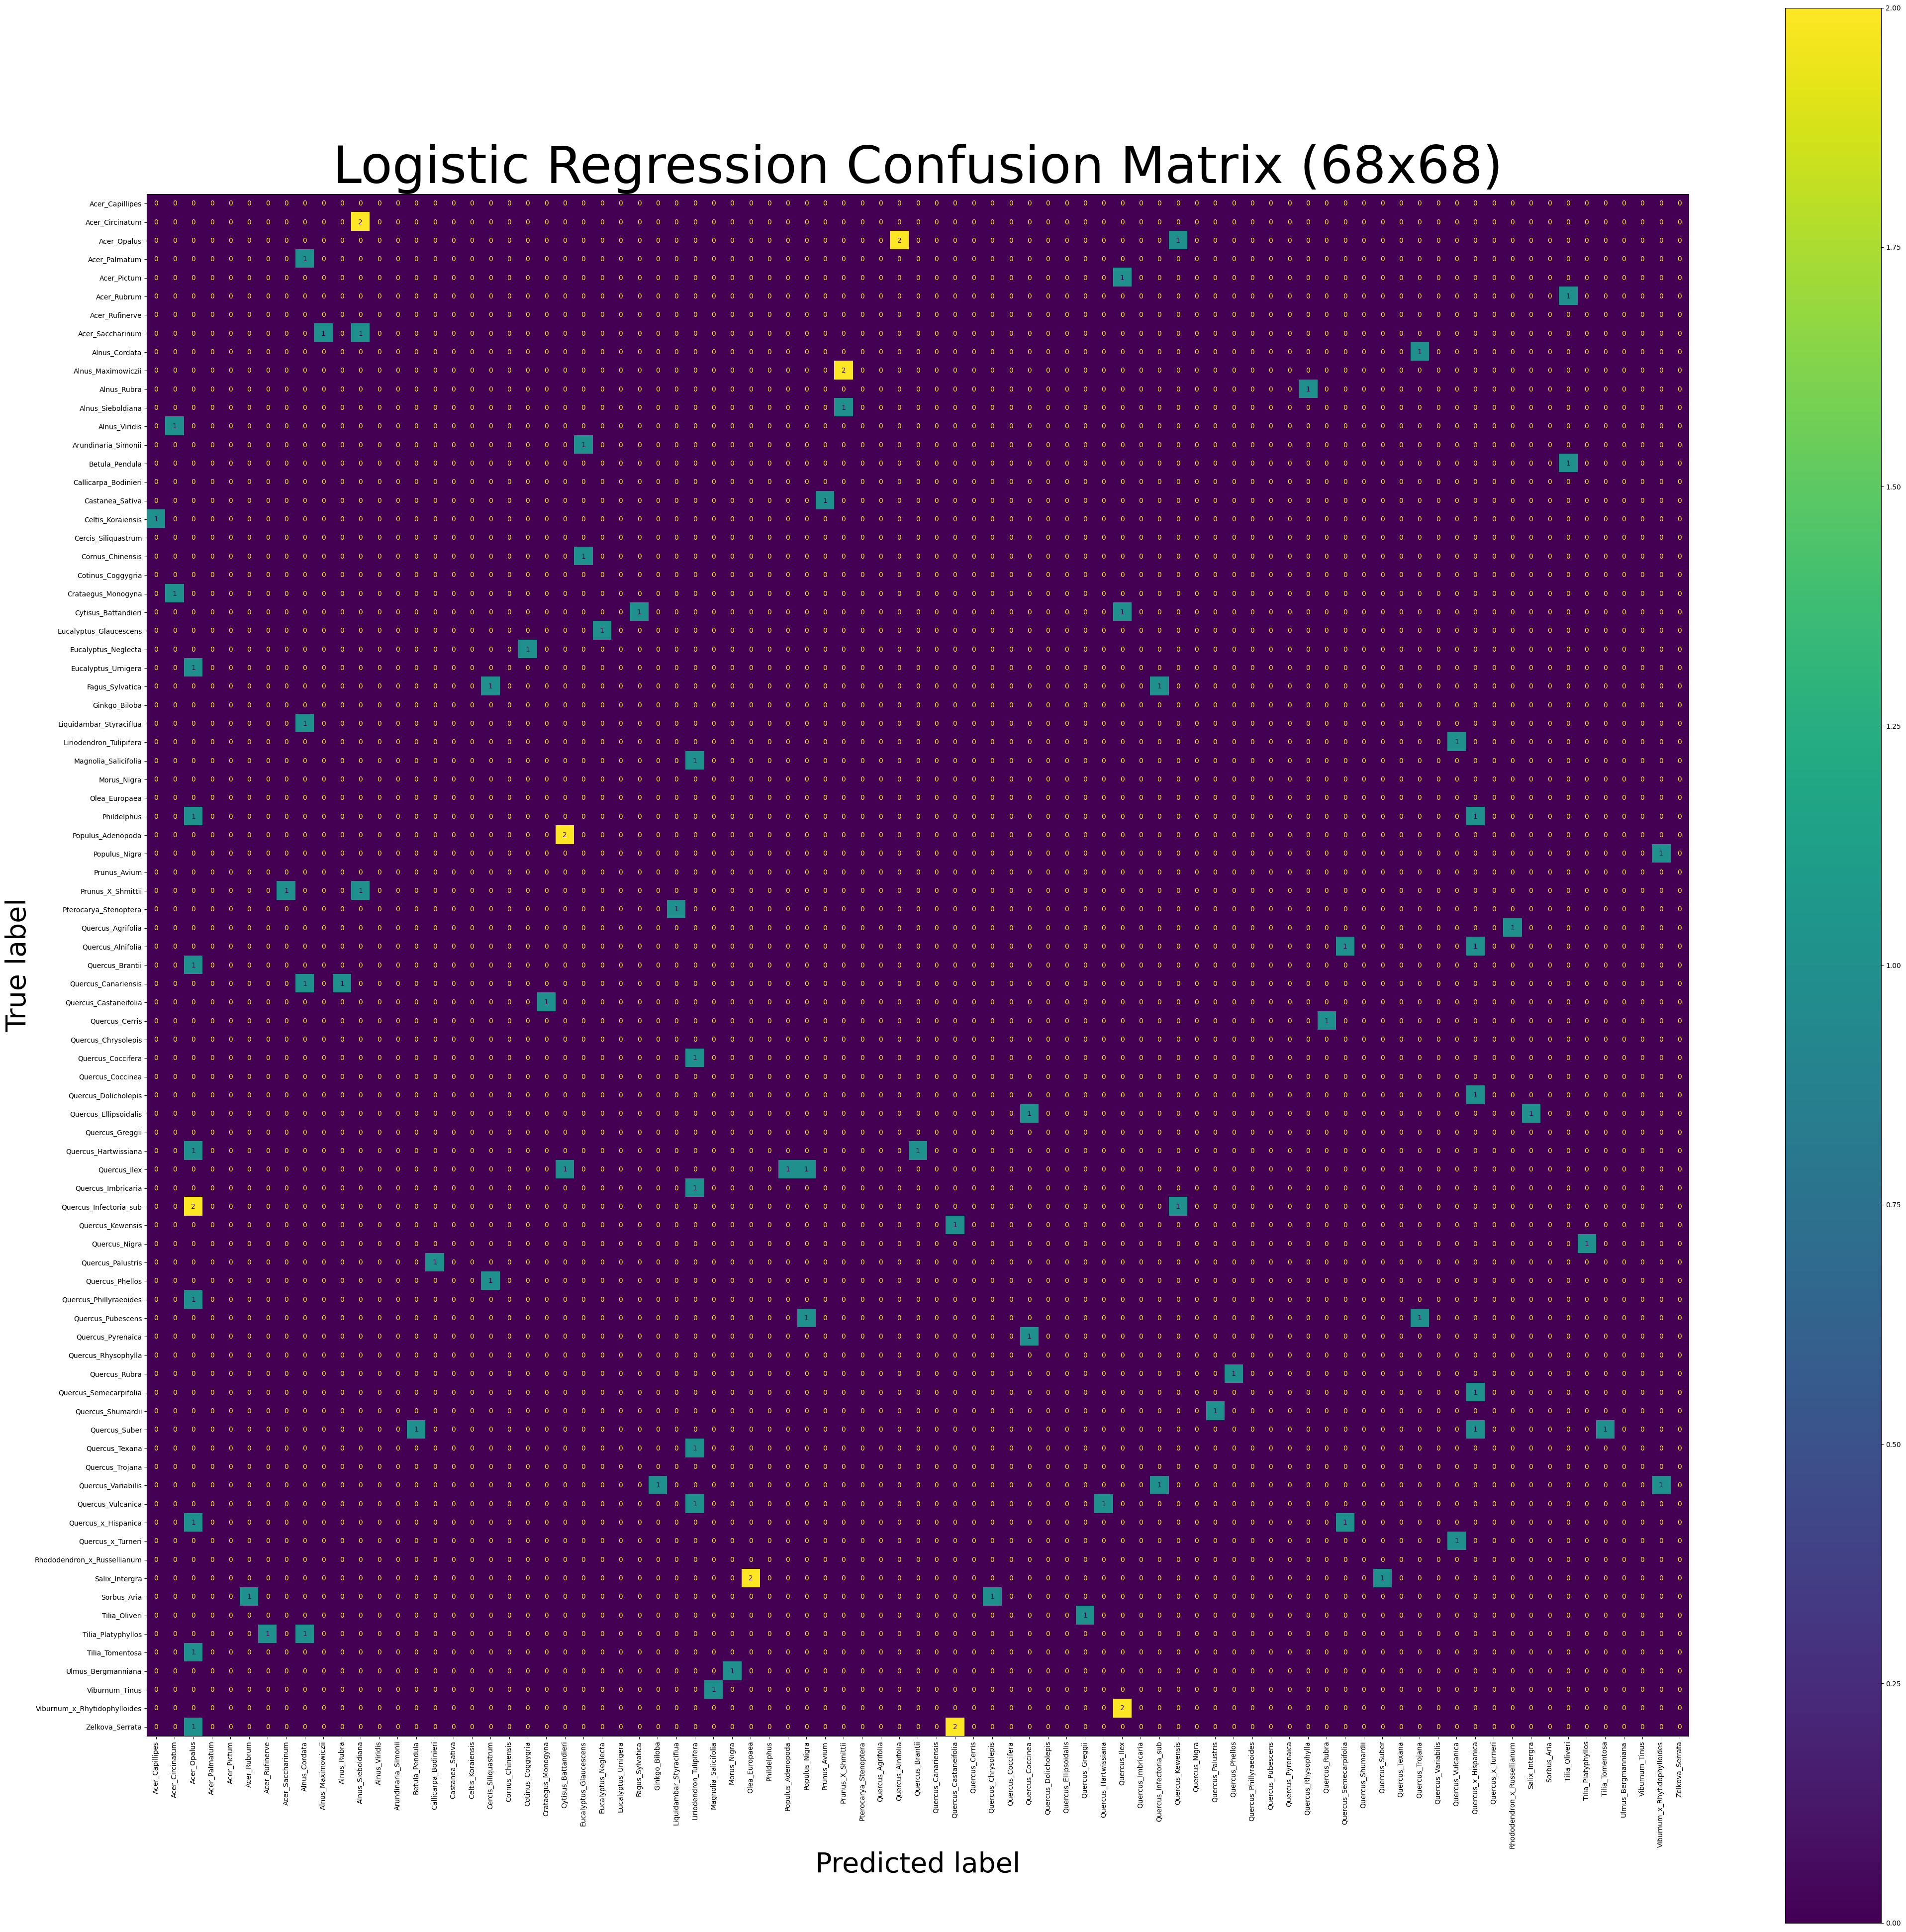
\includegraphics[width=0.7\linewidth]{images/matrix_dt}
\caption{Matrice de confusion du modèle Decision Tree}
\end{figure}

Sans forcément s’intéresser aux labels précis des classes, nous pouvons
observer un grand nombre d’erreurs de prédictions étalées sur différentes
classes, et se reproduisant parfois plusieurs fois pour certaines
classes. Cette vue d’ensemble des mauvaises prédictions confirme les
performances décevantes de notre modèle utilisant l’arbre de décision. 

Ces mauvaises performances peuvent s’expliquer par différents facteurs.
Tout d’abord, on peut pointer le fait que notre jeu de données n’est
sans doute pas le plus optimal, avec 99 classes et seulement 10 échantillons
d’entraînement par classes, l’arbre de décision n’a pas sur construire
un arbre différenciant de façon précise chacune des classes. 

Également, lors du processus de recherche d’hyperparamètres, nous
avons dû le répéter plusieurs fois car les résultats étaient très
fluctuants et il était possible d’avoir des valeurs d’hyperparamètres
optimaux changeantes d’une exécution à l’autre. 

Enfin, les arbres de décisions ont en moyennes des performances plus
basses que d’autres modèles de classification, et sont souvent utilisé
dans le modèle de Random Forest, qui est le prochain modèle que nous
présentons.

\paragraph*{Conclusion}

Pour conclure, le modèle d’arbre de décision n'a pas produit des performances
convaincantes avec notre jeu de données.

Les meilleurs hyperparamètres trouvés sont la profondeur maximale
d’arbre illimitée (None), le nombre minimal d’échantillon pour division
d’un nœud = 5, le critère de division ‘gini’ et enfin le splitter
de type ‘random’, même si pour ce dernier paramètre, il pourrait être
correct d’utiliser le ‘best’. Le tout nous a permis d'obtenir une
précision de 61,5\% sur les données d’entrainement et des valeurs
de métriques de performances allant de 66 à 72\% sur les données de
test.

L’analyse plus précise des hyperparamètres a mis en évidence le fait
que l'absence de limite de profondeur semble préférable, ce qui suggère
que permettre aux arbres de se développer sans restriction conduit
à de meilleurs ajustements aux données d'entrainement.

Pour le nombre minimal d'échantillons requis pour diviser un nœud,
son augmentation a conduit à des performances plus faibles, s'expliquant
par le fait qu'un nombre plus élevé d'échantillons est requis pour
autoriser une division, limitant considérablement le modèle dans sa
caractérisation des 99 classes. Les autres paramètres de critère qualité
et de splitter n’ont pas d’impact significatif sur les performances.

Enfin, les résultats de la matrice de confusion et des boxplots ont
bien souligné la présence fréquente d'erreurs de prédiction, ce qui
peut être attribué à la complexité du problème avec un grand nombre
de classes et un faible nombre d'échantillons par classe. En résumé,
bien que l'arbre de décision soit une approche populaire, les résultats
obtenus soulignent les défis rencontrés dans notre contexte particulier.
Une recherche d’hyperparamètres plus poussée, mais plus demande en
temps de calculs, des données plus riches en nombre d’observations
et des modèles plus sophistiqués comme Random Forest, pourraient être
explorés pour améliorer les performances de classification.

\pagebreak

\subsection{Forêt aléatoire}

Le sixième et dernier modèle de classifications que nous avons choisi
d’utiliser est celui de la forêt aléatoire (Random Forest). Il s'agit
d'une méthode de modélisation qui utilise un ensemble d'arbres de
décision pour résoudre des problèmes de classification avec plusieurs
classes, tout comme dans notre cas. La forêt aléatoire combine les
prédictions de plusieurs arbres de décision individuels, chacun formé
sur un sous-ensemble aléatoire des données d'entraînement. Cette approche
permet de surmonter certaines limitations des arbres de décision individuels,
que nous avons vu précédemment, en réduisant le surajustement et en
améliorant la stabilité des prédictions. L’utilisation du Random Forest
est bien plus répandue que les arbres de décisions simples, en raison
de leur capacité à capturer des relations complexes entre les caractéristiques
et la classe cible grâce à l'agrégation de multiples modèles.

Pour notre classifieur Random Forest, nous avons choisi d’optimiser
les trois hyperparamètres suivants : 
\begin{itemize}
\item Le nombre d'arbres dans la forêt (n\_estimators). 
\item La profondeur maximale de chaque arbre (max\_depth). Une profondeur
à None indique qu'il n'y a pas de restriction sur celle-ci. 
\item Le nombre minimal d'échantillons requis pour diviser un nœud (min\_samples\_split). 
\end{itemize}
Le paramètre n\_estimators est clé. En effet, plus on l’augmente,
plus d’arbres de décisions seront construits et utilisée pour prendre
des décisions lors de la classification. Cependant, plus d’arbres
générés signifie qu’un temps de calcul plus conséquent en sera résultant.
Lors de la recherche d’hyperparamètres, nous nous sommes donc limités
à 5 nombres d’arbres différents : 60, 70, 80, 90 et 100. Cette plage
de valeur a été déterminée par des tests préalables, en observant
des performances d’entraînement satisfaisantes dans cet intervalle. 

Nous avons procédé de même avec le paramètre de profondeur maximale.
Ce paramètre est extrêmement important et impacte fortement les performances
du modèle, observation qui a aussi été faite pour le modèle du Decision
Tree. Les valeurs choisies sont des profondeurs de 2, 5, 7, 100 et
None, c’est-à-dire pas de restriction de profondeur. 

Enfin, le min\_samples\_split est testé pour des valeurs de 2,5 et
10.

Contrairement au Decision Tree, nous avons fait le choix de ne pas
intégrer le critère de division dans les hyperparamètres à optimiser.
En effet, cet hyperparamètre a une influence quasi nulle sur nos résultats
et ajoutait du temps computationnel inutile. Nous avons donc laissé
la valeur par défaut qui fait que le critère utilisé est ‘gini’. 

Après avoir effectué la recherche des meilleurs hyperparamètres, la
meilleure combinaison obtenue pour l’entraînement est la suivante
: max\_depth = None, min\_samples\_split = 5 et n\_estimators = 80
avec un score de précision de 0.917. Les performances obtenues sont
très satisfaisantes. 

Concernant la profondeur maximale des arbres, on observe que l'absence
de limite de profondeur (None) semble être plus avantageuse. Cela
suggère que permettre aux arbres de se développer sans contrainte
de profondeur conduit à de meilleures performances dans notre cas.
Par conséquent, il est tout à fait normal que, avec cette liberté
en ce qui concerne la profondeur, le modèle s'ajuste de manière optimale
aux caractéristiques des données d'entraînement. De plus, cette approche
semble particulièrement pertinente étant donné le grand nombre de
classes présentes dans notre jeu de données. 

Afin de mieux visualiser l’importance de cet hyperparamètre ainsi
que du nombre d’estimateurs, nous avons fait le choix de représenter
les courbes de performance des différentes combinaison d’hyperparamètre
lorsque min\_samples\_split = 5 : 

\begin{figure}[h]
\centering{}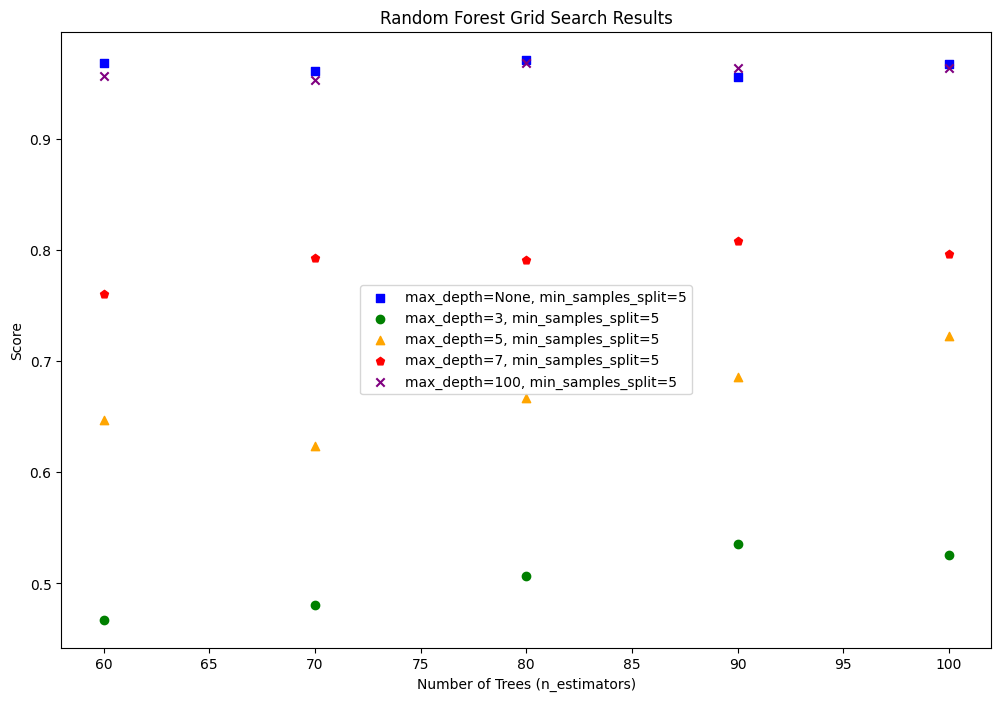
\includegraphics[width=0.7\linewidth]{images/courbe_rf}
\caption{Courbe de score du modèle Random Forest pour différents hyperparamètres}
\end{figure}

Tout d’abord, nous observons que le paramètre le plus impactant sur
les performances d’entrainement du modèle est la profondeur maximale
d’arbre. En, effet, on voit une très nette différence de performance
entre 3,5, 7 et 100 niveaux de profondeurs, avec quasiment 0.2 de
score d’écart. La différence entre 100 et une profondeur illimitée
est par contre quasiment inexistante, supposant que la valeur None
s’approche des valeurs proches de la centaine. On a donc une augmentation
pouvant s’apparenter à une croissance logarithmique. Les explications
faites précédemment sur ce paramètre justifient les résultats obtenus. 

Pour ce qui est nombre d’arbres générés par notre modèle, nous observons
une croissance du score, mais très faible, plus ce nombre est élevé.
Cette observation montre que l’on se trouve dans un intervalle de
valeurs assez optimale. Cela signifie qu’un nombre d’arbres entre
60 et 100 permet de très bien décrire et caractériser notre jeu de
données. 

Pour réellement mesurer les performances du meilleur modèle sur l’ensemble
d’entrainement, nous l’évaluons sur un ensemble de test composé de
données que le modèle n’a jamais rencontré. Voici les valeurs moyennes
des métriques de performances obtenues pour chaque classe : 
\begin{itemize}
\item Précision : 97,811 \textpm{} 7,490 \% 
\item Rappel : 97,306 \textpm{} 9,131 \% 
\item F1-score : 97,249 \textpm{} 7,212 \% 
\end{itemize}
Nous traçons également les boxplots correspondants : 

\begin{figure}[h]
\centering{}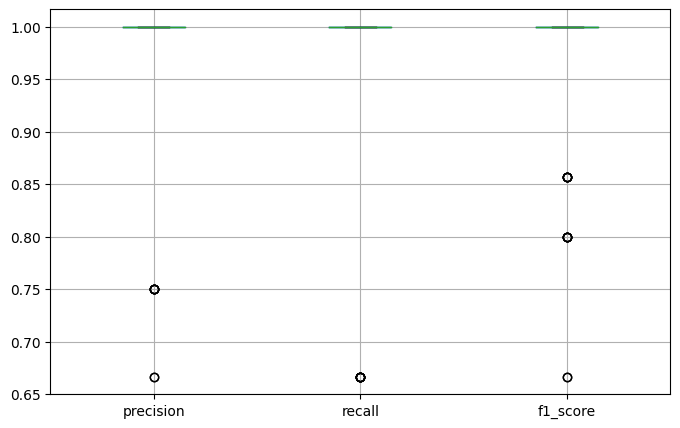
\includegraphics[width=0.7\linewidth]{images/boxplot_rf}
\caption{Distribution des métriques d’évaluation pour le modèle Random Forest}
\end{figure}

Premièrement, on remarque que les valeurs des 3 métriques de performances
sont excellentes, étant toutes entre 97 et 98\%. Le modèle a donc
très bien performé sur les données de test. Comme on peut le voir
dans les boxplots, les prédictions sont correctes pour la quasi-totalité
des classes, avec seulement très peu de valeurs aberrantes (outliers).
Les boxplots sont en effet quasiment invisibles et tous au niveau
de la valeur 1 pour les trois métriques de performances. Il existe
cependant des classes pour lesquelles le modèle a moins bien performé.
Au total, seulement 14 classes sur les 99 ont un f1-score non parfait,
c’est-à-dire différent de 1. Cela n’est absolument pas alarmant sur
les performances de notre modèle, mais indique que des points d’améliorations
subsistent pour parfaire notre modèle, bien que déjà très performant.
Enfin, nous dressons la matrice de confusion qui montre toutes les
erreurs de prédictions, en affichant les couples de classes où une
classe prédite était différente de la classe réelle, avec le nombre
d’occurrences. 
\begin{figure}[h]
\centering{}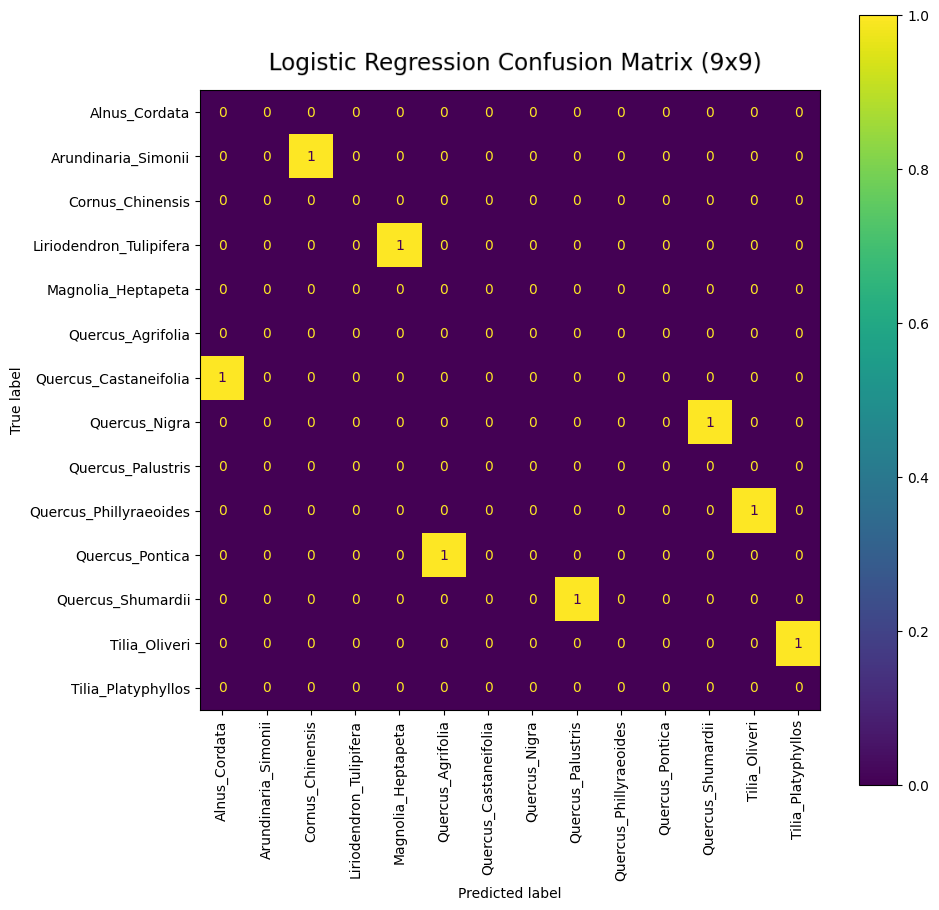
\includegraphics[width=0.7\linewidth]{images/matrix_rf}
\caption{Matrice de confusion du modèle Random Forest}
\end{figure}

Comme observé précédemment via les métriques de performances, nous
voyons que les erreurs de prédictions sont très rares et ne sont pas
concentrées sur une classe en particulier.

\paragraph*{Conclusion}

Pour conclure, le modèle de régression Random Forest s’est révélé
très performant pour résoudre notre problème de classification. 

Les meilleurs hyperparamètres trouvés sont la profondeur max\_depth
= None, le nombre minimal d'échantillons requis pour division min\_samples\_split
= 5 et le nombre d’arbres de la forêt n\_estimators = 80, avec un
score de précision de 91,7\% sur les données d’entraînement, et des
métriques de performance allant de 97 à 98\% sur les données de test. 

En analysant les courbes de performances en fonction de la profondeur
maximale et du nombre d'estimateurs, nous avons constaté que la profondeur
maximale a un impact significatif sur les performances d'entraînement.
Pour le nombre d'arbres, bien que le score augmente avec leur nombre,
la croissance est faible, suggérant un intervalle optimal entre 60
et 100 arbres. L'évaluation sur un ensemble de test montre des performances
très satisfaisantes, avec des moyennes de précision, rappel et f1-score
toutes supérieures à 97\%. Les boxplots associés confirment la robustesse
du modèle, avec très peu de valeurs aberrantes. Seules 14 classes
sur 99 présentent des f1-scores non parfaits, indiquant des points
d'amélioration possibles malgré la performance globalement élevée
du modèle. 

En examinant la matrice de confusion, nous constatons que les erreurs
de prédiction sont rares et dispersées, attestant de la qualité du
modèle Random Forest dans notre contexte. En conclusion, notre modèle
Random Forest s’est montré très performant et efficace pour notre
jeu de données, s’adaptant parfaitement à la grande diversité de classes
existantes. La flexibilité que donnée par l’absence de profondeur
d’arbre a joué un rôle important pour arriver aux performances obtenues,
en plus de la robustesse habituelle d’une méthode telle que Random
Forest.

\pagebreak

\section{Conclusion}
\begin{center}
\begin{figure}[h]
\begin{centering}
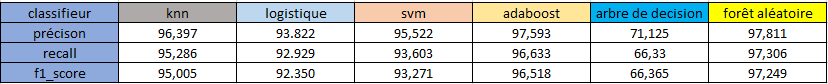
\includegraphics[scale=0.6]{images/recap} 
\par\end{centering}
\caption{\label{fig:adaboost-evaluation}tableau récapitulatif des performances
globales des différents classifieurs }
\end{figure}
\par\end{center}

Comme on peut le voir sur le tableau récapitulatif ci-dessus, la forêt
aléatoire présente les meilleurs performances suivi de peu par l'adaboost
pour notre jeu de données, l'arbre de décision lui n'est adapté. Cela
dit, chaque classifieurs possède ses forces et ses faibles et c'est
à travers de la nature de nos données que l'on doit chercher le plus
optimal pour le problème de classification.
\end{document}
